\chapter{Theoretische Grundlagen}
\label{ch:theorie}

Kongruenz ist ein syntaktisches Phänomen, das sich in morphologischer
Markierung ausdrückt. \citet{corbett2006} richtet sich in seiner
Arbeitsdefinition nach \citet[610]{steele1978}, die Kongruenz als eine
irgendwie geartete systematische Kovarianz zwischen einer semantischen oder
formalen Eigenschaft eines Elements und einer formalen Eigenschaft eines
anderen definiert.%
%
	\footnote{\blockcquote[610]{steele1978}{The term \emph{agreement} commonly
		refers to some systematic covariance between a semantic or formal
		property of one element and a formal property of another}.%
	}
%
Hervorzuheben ist dabei der Begriff der Kovarianz. Informationen über den Kopf
einer Phrase zeigen sich an einem anderen Wort, das sich auf diesen Kopf
bezieht. Dies kann im Fall eines Substantivs ein Modifizierer des Substantivs
sein, der mit diesem in seinen grammatischen Merkmalen übereinstimmt, zum
Beispiel ein Adjektiv oder ein Artikel, oder auch ein anderer Kopf, der
anaphorisch von diesem Substantiv abhängt, wie ein Pronomen. Kongruenz zeigt
sich daneben auch in der Übereinstimmung des Verbs in Person und Numerus mit
seinem Subjekt. \citet[20]{corbett2006} fasst die Kongruenzrelation lakonisch
als \textquote{essentially a matter of \q{displaced} information} zusammen. Die
unterschiedlichen Grammatiktheorien haben verschiedene Auffassungen davon, wie
Kongruenz zustande kommt, beziehungsweise davon, wie sie formal zu modellieren
ist \autocite[siehe~z.\,B.][]{mueller2023}. \citeauthor{corbett2006} beschreibt
das Phänomen aus morphologischer und typologischer Perspektive.

\section{Controller, Target und Domäne}
\label{sec:ctrltarg}

Wichtige Begriffe im Hinblick auf Kongruenz nach \citet{corbett2006} sind
zunächst \fw{Controller} (Kongruenzauslöser) und \fw{Target} (Kongruenzziel).%
%
	\footnote{In der deutschsprachigen Fachliteratur finden sich verschiedene
	Terminologien. \citet{fleischerschallert2011} sprechen beispielsweise von
	\q{Kongruenzträger} und \q{-ziel}, \citet{panther2009} von
	\q{Kontrolleur} und \q{Ziel}.}
%
Dieses Begriffspaar bezeichnet die beiden zuvor genannten, in bestimmten
grammatischen Merkmalen übereinstimmende Instanzen, die in einer
Kongruenzrelation zueinander stehen. Die Kongruenzrelation geht vom Controller
aus, nach \citeauthor{corbett2006} \q{empfängt} das Target die Information zu
dessen grammatischen Merkmalen sozusagen.

\begin{figure}
\centering
	\begin{tabular}[t]{l @{} l c}
		\itshape{grün}
		& \itshape{-er}
		& \itshape{Baum}
		\\

		%
		& \colorbox{gray}{\textcolor{white}{-\textsc{nom.m.sg}}}
		& \textcolor{gray}{\textsc{nom.m.sg}}
		\\

		\cmidrule(lr){1-2}
		\cmidrule(lr){3-3}

		\mc{2}{c}{\textsc{target}}
		& \mc{1}{c}{\textsc{controller}}
		\\

		\mc{2}{c}{\tikzmark{ctrltarg_targ}}
		& \mc{1}{c}{\tikzmark{ctrltarg_ctrl}}
		\\
	\end{tabular}
\begin{tikzpicture}[remember picture, overlay]
\draw [myarrow]
	([yshift=2.5ex]{pic cs:ctrltarg_ctrl})
	|- ++ (south:2ex) -|
	([yshift=2.5ex]{pic cs:ctrltarg_targ})
	node [near start, below] {\smaller[1]\scshape kongruenz};
\end{tikzpicture}
\caption{\q{Verschobene} Information in einer Kongruenzrelation}
\label{fig:ctrltarg}
\end{figure}

Das Beispiel in \figref{fig:ctrltarg} enthält ein Substantiv, \fw{Baum}. Von
diesem ist bekannt, dass es die folgenden grammatischen Merkmale trägt:
maskulin, Singular. Ferner sei angenommen, dass es im Nominativ steht. Die
Merkmale \fw{maskulin} und \fw{Singular} sind dem Lexikoneintrag des Wortes
inhärent; sie werden nicht morphologisch an ihm markiert. Die grammatischen
Informationen zeigen sich jedoch in einem Portmanteau-Morphem zusätzlich zum
Kasus des Substantivs als Suffix \fw{-er} am Adjektiv \fw{grün}, das von sich
aus keine Personenmerkmale und Informationen zum Kasus der Nominalphrase (NP)
enthält. Personen- und Kasusmerkmale des Substantivs werden durch die Flexion
am Adjektiv widergespiegelt und erscheinen daher \q{verschoben}. Das Adjektiv
ist damit das Target der Kongruenz\-relation, während das Substantiv den
Controller darstellt.

Bei Kongrenz geht es im Grunde also um die Vererbung beziehungsweise das Teilen
grammatischer Merkmale (\fw{grammatical features}; \cite{corbett2012}). Bei
Personenbezeichnungen sind Informationen zum Genus und Numerus tendenziell an
semantische Eigenschaften der bezeichneten Person gebunden; bei Dingen und
Abstrakta ergeben sie sich anhand formaler Kriterien \autocites[vgl.][2--4,
125--132]{corbett2006}{koepckezubin2017}. So bezeichnet \fw{Mutter} eine
\textquote{Frau, die ein oder mehrere Kinder geboren hat}, oder allgemeiner
eine \blockcquote[s.\,v.~\fw{Mutter}]{duden-online}{Frau, die in der Rolle
einer Mutter ein oder mehrere Kinder versorgt, erzieht}. \fw{Mutter} hat damit
\emph{feminin} als Wert des grammatischen Merkmals Genus. Doch dass etwa
\fw{Baum} maskulin und \fw{Liebe} feminin ist, hat kein Korrelat in der
außersprachlichen Realität, sondern ist eine Konvention des
Deutschen\il{Neuhochdeutsch}.%
%
	\footnote{Nichtsdestoweniger ist die Genuszuweisung bei Inanimata nicht
		ganz willkürlich. \citeauthor{koepckezubin2017} haben seit den 1980er
		Jahren gezeigt
		\autocites[z.\,B.][]%
			{koepcke1982}%
			{koepckezubin1996}%
			{koepckezubin2009}%
			{koepckezubin2017},
		dass nicht nur Derivationssuffixe wie
			\fw{-ling} (\textsc{m}),
			\fw{-schaft} (\textsc{f}) oder
			\fw{-chen} (\textsc{n}),
		sondern auch die phonologische Struktur von Wortstämmen und die
		Zugehörigkeit von Substantiven zu bestimmten semantischen Feldern einen
		starken Einfluss auf die Genuszuweisung haben. Zum Beispiel tendieren
		konsonantenreiche Einsilber zum Maskulinum (%
			\fw{der} /braɪ̯/,
			/ɛrnst/,
			\smash{/ʃtrʊmp͡f/}%
			% , aber
			% \fw{die} /ʃprɔʏ̯/,
			% \fw{das} /fɔlk/,
			% \fw{die} /frɪst/
			;
		\cite[vgl.][475--479]{koepckezubin1996}), während Zweisilber, die auf
		Schwa enden, häufig dem Femininum zugeordnet werden (%
			\fw{die} /liːbə/,
			\smash{/ʃprɪt͡sə/,}
			/taʃə/%
			% , aber
			% \fw{der} /kɛːzə/,
			% \fw{das} /aʊ̯ɡə/
			;
		\cite[vgl.][207--209]{koepckezubin2017}). Was semantischer Felder
		betrifft, sind zum Beispiel Sprachbezeichnungen gewöhnlich Neutra (%
			\fw{das Deutsche},
			\fw{Hindi},
			\fw{Nahuatl};
		\cites[siehe]%
			[480]{koepckezubin1996}%
			[137--139]{koepckezubin2009}%
			[210--214]{koepckezubin2017}
		für weitere Beispiele aus anderen Feldern).%
		\label{fn:koepckezubin}
	}

Wie darüber hinaus aus dem Schema in \figref{fig:termini} deutlich wird,
unterscheiden \citet{wechslerzlatic2003} nicht nur zwischen grammatischer und
pragmatischer Kongruenz, sondern innerhalb der grammatischen Kongruenz noch
Kongruenz mit den Merkmalskategorien Concord (grammatische Kongruenz
\fw{ad formam} innerhalb der NP) und Index (grammatische Kongruenz
\fw{ad formam} oder \fw{ad sensum} außerhalb der NP;
\cite[8--17]{wechslerzlatic2003}. Die theoretische Grundlage für diese
Unterscheidung liefert ihnen die \fw{Head-driven Phrase Structure Grammar}
(HPSG; \cite{pollardsag1994}). Im Gegensatz zu der Anmerkung von
\citet[164]{fleischer2012}, dass \q{formal} und \q{semantisch} in der Forschung
synonym zu \q{grammatisch} und \q{pragmatisch} benutzt werden, unterscheiden
\citet{wechslerzlatic2003} also alle vier Termini. Pragmatische und semantische
Kongruenz überschneiden sich mit dem Begriff \fw{constructio ad sensum}, da sie
sich beide aus der Semantik speisen.

\begin{figure}
\centering
\begin{tikzpicture}[baseline=(grm.base), shorten >= 4pt, shorten <= 4pt]
	\node [draw, rectangle, align=center] (frm) at (0,0) {
		formal\\ \footnotesize (\fw{ad formam})
	};
	\node [draw,rectangle, align=center] (sem) at (3,0) {
		semantisch\\ \footnotesize (\fw{ad sensum})
	};
	\node [draw, rectangle] (grm) at (0,2) {grammatisch};
	\node [draw, rectangle] (prg) at (3,2) {pragmatisch};
	\draw [-latex] (grm) -- (frm);
	\draw [-latex] (grm) -- (sem);
	\draw [-latex] (prg) -- (sem);

	\node [draw, rectangle, align=center, gray] (con) at (0,-2) {
		\textsc{concord} \\
		\footnotesize (Modifikatoren)
	};
	\node [draw, rectangle, align=center, gray] (idx) at (3,-2) {
		\textsc{index} \\
		\footnotesize (anaphorische\\
		\footnotesize Bindung)
	};
	\draw [-latex, gray] (con) -- (frm);
	\draw [-latex, gray] (idx) -- (frm);
	\draw [-latex, gray] (idx) -- (sem);
\end{tikzpicture}
\caption%
	[Einteilung der Kongruenztypen und beteiligte Merkmale nach Wechsler~\&~%
	Zlatić]%
	{Einteilung der Kongruenztypen und beteiligte Merkmale nach
	\citet{wechslerzlatic2003}}
\label{fig:termini}
\end{figure}

Ein weiterer wichtiger Faktor in der Chrakterisierung von Kongruenzbeziehungen
nach \citet{corbett2006} ist die Domäne. Dieser Begriff wird von
\citet{corbett2006} nicht formal definiert. Aus seinen Ausführungen ist aber zu
entnehmen, dass damit der Abstand zwischen Controller und Target im Sinne der
Konstituenz von Sätzen gemeint ist. So gibt es nach \citet[54]{corbett2006}
vier Domänen mit wachsender Lokalität und abnehmender Kanonizität:

\begin{enumerate}[noitemsep]
	\item innerhalb der NP;
	\item außerhalb der NP aber innerhalb des Teilsatzes;
	\item außerhalb des Teilsatzes aber innerhalb des Satzes;
	\item außerhalb des Satzes.
\end{enumerate}

In (\ref{ex:beidedomains_1}--\ref{ex:beidedomains_4}) wird jeweils ein Beispiel
pro Domäne gegeben. In \REF{ex:beidedomains_1} stellt \lit{bede} `beide' als
Target einen Modifikator seines Controllers \lit{wingarten} `Weingarten' in
derselben NP beziehungsweise in derselben Nominalgruppe dar. Das Target steht
attributiv zum Controller.

\begin{exe}
\ex \label{ex:beidedomains_1}
	\gll die bede wingarten \\
		die beide-\textsc{acc.pl.m.st} Weingarten-\textsc{acc.pl.m} \\
	\trans `die beiden Weingärten'
		\parencites%
			(Nr.~1221, Zürich, 1290)%
			[484,9]{cao2}
\end{exe}

Der Controller \lit{zil} `Ziele, Fristen' in \REF{ex:beidedomains_2} bildet
den Kopf der in sich abgeschlossenen Genitiv-NP \lit{der vor genanten zil} `der
vorgenannten Ziele'. \textins{\lit{B}}\lit{eidiv} `beide' als darauf bezogenes
Target steht außerhalb davon als Kopf der darüber liegenden NP, aber dennoch im
gleichen Satzteil wie \lit{zil} `Ziele, Fristen', da die komplexe NP
\lit{der vor genanten zil / ainez / oder beidiv} `eines oder beide der
vorgenannten Ziele' das Akkusativobjekt zu \lit{verſitzzet} `versäumt'
ist. Das Target steht in einer anaphorischen Beziehung zum Controller.

\begin{exe}
\ex \label{ex:beidedomains_2}
	\gll ſwenne man der {vor genanten} zil / ainez / oder
		beidiv \textelp{} verſitzzet \\
		so=wenn man der vorgenannten Ziel[\textsc{gen.pl.n}] {} eines {}
		oder beide-\textsc{acc.pl.n.st} {} versäumt \\
	\trans `falls man eines oder beide der vorgenannten Ziele \textelp{}
		versäumt'
		\parencites%
			(Nr.~619, Augsburg, 1283)%
			[47,31]{cao2}
\end{exe}

In \REF{ex:beidedomains_3} ist das Target \lit{beideu} `beide' auf den
Controller \lit{rihtær} `Richter' bezogen, befindet sich formal aber nicht im
gleichen Satzteil wie dieser, dennoch aber im gleichen (Teil-)Satz, insofern
beide NPs vom gleichen Verb \lit{ſprachen} `sprachen' abhängen. Auch hier ist
die Kongruenzbeziehung anaphorisch.

\begin{exe}
\ex \label{ex:beidedomains_3}
	\gll Die rihtær ſprachen beideu {dar zuͦ} \\
		die Richter[\textsc{nom.pl.m}] sprachen beide-\textsc{nom.pl.n.st}
			dazu \\
	\trans `die Richter äußerten sich beide dazu'
		(%
			B1: 28ra,8;
			vgl.~\KC: V.~10090; \cite[267]{schroeder1895}%
		)
\end{exe}

Im letzten Schritt bezieht sich das Target \lit{bede} `beide' in
\REF{ex:beidedomains_4} zwar auf \lit{herren} `Herren', doch bildet
\lit{herren} das Subjekt zum Verb \lit{lident} `leiden', während
\lit{bede} zusammen mit dem Personalpronomen \lit{Si} `sie' das
Subjekt von \lit{ligent} `liegen' bildet. Damit stehen der (Erst-)Controller
\lit{herren} und das Target \lit{bede} in unterschiedlichen Sätzen. Das
\norm{bėide}-Target bezieht sich ebenfalls anaphorisch auf seinen Controller.

\begin{exe}
	\ex \label{ex:beidedomains_4}
		\gll Min herren lident ovch groze not. \\
			mein Herr-\textsc{nom.pl.m} leiden auch große Not \\
	\sn \gll Si ligent bede fvͤr tot \\
			\textsc{3pl\subM.nom} liegen beide-\textsc{nom.pl.m.st} für tot \\
	\trans `Meine Herren leiden auch große Not. Sie liegen beide tot
		\textins{darnieder}.'
		(%
			VB: 86ra,3--4;
			vgl.~\KC: V.~12033--12034; \cite[301]{schroeder1895}%
		)		
\end{exe}

\section{Index und Concord}
\label{sec:indexconcord}

\phantomsection
\label{phsec:index}
Das Merkmal Index ist in der HPSG seinerseits Teil des Merkmals Content eines
lexikalischen Zeichens, das sich aus der Semantik speisende Informationen über
dessen Denotat enthält, konkret also grammatikalisierte Personen\-merkmale wie
Person, Numerus und Genus \autocite[15--17]{wechslerzlatic2003}. Auch in der
mit der HPSG verwandten \fw{Lexical-Functional Grammar} (LFG;
\cites{kaplanbresnan1982}{bresnan2001}{bresnanetal2016}) existiert ein solches
Merkmal \autocite[189--190]{bresnanetal2016}. Das Index-Merkmal bildet die
Basis für anaphorische Referenz, indem es ein Individuum oder ein Ding als
Instanz des Bezeichneten im Diskurs verankert
\autocite[10--11]{wechslerzlatic2003}. Während eine große Nähe zwischen
Index und Semantik konstatiert wird, ist diese nicht absolut, da auch das
generische Pronomen \fw{man} oder das expletive Subjektspronomen \fw{es} einen
Index besitzen, obwohl sie sich nicht auf eine bestimmte semantische Größe
beziehen \autocite[11--13]{wechslerzlatic2003}. Dies wird bei der Konjugation
von Verben und der Bindung von Reflexivpronomen sichtbar
\REF{ex:explvbkonj}.

\begin{exe}
\ex \label{ex:explvbkonj}
	\begin{xlist}
	\ex Es\tsub{i} regnet\tsub{i}.
	\ex Man\tsub{i} kann\tsub{i} es sich\tsub{i} vorstellen.
	\end{xlist}
\end{exe}

\citet{kingdalrymple2004} argumentieren des Weiteren, dass Index in
koordinierten nominalen Strukturen ein nicht-distributives Merkmal darstellt,
indem die Kombination zweier Substantive einen neuen Index erhält, mit dem
kongruiert wird \autocite[74--76]{kingdalrymple2004}. \fw{Jan} und \fw{Markus}
in \REF{ex:coordidx} haben zwar jeder für sich einen Singular-Index, die Gruppe
\fw{Jan und Markus} hat aber einen Plural-Index, was sich in der Kongruenz
zwischen Subjekt und Verb zeigt.

\begin{exe}
\ex\label{ex:coordidx}
\begin{xlist}
	\ex[]{[Jan\tsub{i} und Markus\tsub{j}]\tsub{k} spielen\tsub{k} Fußball.}
	\ex[*]{Jan\tsub{i} und Markus\tsub{j} spielt\tsub{{i/j}} Fußball.}
\end{xlist}
\end{exe}

\phantomsection
\label{phsec:concord}
Das Gegenstück zum Index bildet Concord, das in der HPSG Teil des Kopfmerkmals
ist \autocite[17]{wechslerzlatic2003}. Das Merkmal Concord existiert ebenso in
der LFG \autocite[189--192]{bresnanetal2016} und enthält in beiden
Theoriesystemen syntaktisch relevante Informationen über den nominalen
Phrasenkopf, die im Deutschen\il{Neuhochdeutsch} für einzelne, unkoordinierte
NPs weitgehend deckungsgleich mit denen des Index sind:%
%
	\footnote{\citet{wechslerzlatic2003} untersuchen den Fall des
	Bosnisch-Kroatisch-Mazedonisch-Serbischen (\ili{BKMS}), in dem es
	Substantive gibt, für die dies nicht der Fall ist.}
%
Zu den Merkmalen Numerus und Genus tritt das strukturelle Merkmal Kasus, dafür
spielt Person hier keine Rolle. Kongruenz über das Merkmal Concord herrscht
typischerweise zwischen einem nominalen Kopf und seinen Modifizierern, was in
der HPSG mit dem \fw{Head Feature Principle} begründet wird. Dieses besagt im
Grunde, dass ein Phrasenkopf seine grammatischen Informationen mit seinen
Töchtern teilt \autocite[vgl.][22]{wechslerzlatic2003}. Daher ist im Gegensatz
zum Index das Merkmal Concord lokal auf die NP beschränkt, während das
Index-Merkmal überall dort vorkommt, wo anaphorische Bindung eine Rolle spielt
\parencites[14--16, 22]{wechslerzlatic2003}[189]{bresnanetal2016}.

In Bezug auf koordinierte Substantive wie in \REF{ex:coordidx} sei angemerkt,
dass \citet[76--78]{kingdalrymple2004} Concord im Gegensatz zum Index als
distributives Merkmal analysieren. Dies bedeutet, dass Modifizierer von
koordinierten Substantiven mit jedem Konjunkt einzeln in Concord-Merkmalen
übereinstimmen müssen, um einen akzeptablen Ausdruck zu produzieren. Das
Beispiel in \REF{ex:engartdiscong} illustriert dies, insofern \fw{these}
`diese' nur dann verwendet werden kann, wenn beide von ihm determinierten
Konjunkte jeweils im Plural stehen \REF{ex:engartdiscong_1} oder wenn es
lediglich ein einzelnes Substantiv determiniert und stattdessen die Konjunktion
auf höherer syntaktischer Ebene stattfindet
\REF{ex:engartdiscong_4}.

\begin{exe}
\ex\label{ex:engartdiscong}
	\langinfo%
		{Englisch}
		{}
		{\cite[nach][70]{kingdalrymple2004}}
	\begin{xlist}
	\ex[]{these{\ob}\textsc{pl}{\cb} boys{\ob}\textsc{pl}{\cb}
		and girls{\ob}\textsc{pl}{\cb}}
		\label{ex:engartdiscong_1}
	\ex[*]{these{\ob}\textsc{pl}{\cb} boys{\ob}\textsc{pl}{\cb}
		and girl{\ob}\textsc{sg}{\cb}}
		\label{ex:engartdiscong_2}
	\ex[*]{this{\ob}\textsc{sg}{\cb} boy{\ob}\textsc{sg}{\cb}
		and girls{\ob}\textsc{pl}{\cb}}
		\label{ex:engartdiscong_3}
	\ex[]{these{\ob}\textsc{pl}{\cb} boys{\ob}\textsc{pl}{\cb}
		and this{\ob}\textsc{sg}{\cb} girl{\ob}\textsc{sg}{\cb}}
		\label{ex:engartdiscong_4}
	\end{xlist}
\end{exe}

\section{Genus, Sexus und Belebtheit}
\label{sec:gendsex}

Wenn im Folgenden von \textit{Genus} die Rede ist, bezeichnet der Begriff das
grammatische Geschlecht eines Substantivs. Da es sich beim
Mittelhochdeutschen\il{Mittelhochdeutsch} um eine flektierende Sprache handelt,
ist die häufig zitierte Definition von \citet[231]{hockett1958} relevant, die
Genera relational begreift als Klassen von Substantiven, die sich im Verhalten
von darauf bezogenen Wörtern zeigen.%
%
	\footnote{\foreigntextcquote{english}[231]{hockett1958}{Genders are classes
		of nouns reflected in the behavior of associated words}.}
%
Genus wird also als grammatische Kategorie der Klassifizierung von Substantiven
aufgefasst, die an der Kongruenzform von darauf bezogenen Targets erkennbar
ist. Im Sinne \posscite[62--63]{corbett1991} bezieht sich diese Definition auf
\fw{covert gender}, bei dem die Klassenzugehörigkeit eines Substantivs nicht
aus seiner Form erschlossen werden kann. Wie zum Beispiel von
\citet{koepckezubin2017} gezeigt, besitzt das Deutsche\il{Neuhochdeutsch}
allerdings durchaus Aspekte overter Genuszuweisung, sei es durch die Semantik
des Bezeichneten, die Zugehörigkeit zu einer bestimmten Klasse von Dingen oder
die phonologische Struktur des Lexems.

Von den 257 von \citet{corbett2013b} untersuchten, typologisch diversen
Sprachen besitzen 84 (32,7\,\%) ein sexusbasiertes System als semantische
Grundlage der Klasseneinteilung; in den Daten von \tit{Grambank}
\autocite{skirgardetal2023} fällt dieser Wert auf lediglich 410 von 2.206
Varietäten (18,6\,\%; \cite[siehe][]{haynie:gb051}). Gerade der Aspekt der
Sexusbasiertheit führt zu einiger Komplexität beim Zusammenspiel von Geschlecht
im biologischen und soziokulturellen Sinn sowie der sekundären Nutzung von
Geschlecht als grammatischer Kategorie \autocites[dazu
ausführlich][]{kotthoffnuebling2018}{steriopolosteriopolo2022}. Die
Doppeldeutigkeit von \fw{gender} im Englischen\il{Englisch} als Bezeichnung
einerseits für das soziale Geschlecht und die damit verbundene
Geschlechter\-rollen\-praxis und andererseits für die grammatische Kategorie
verkompliziert tendenziell den Diskurs, indem zwei miteinander interagierende
Ebenen terminologisch vermischt werden.

Der Zusammenhang von sozialem Geschlecht und Sprache führt immer wieder zu
stark emotional geführten, sprachästhetisch bis sozialkritisch motivierten
Debatten insbesondere über die Notwendigkeit der expliziten sprachlichen
Sichtbarmachung von Frauen durch Movierung der maskulinen Form eines Nomen
Agentis sowie von Personen, die sich dem queeren Spektrum zugehörig fühlen,
durch weitere typografische Mittel \autocite[dazu kritisch
resümierend][]{kasper2022}. Mit \citet[61--89]{kotthoffnuebling2018} ist
anzumerken, dass der Laiendiskurs um das sogenannte \q{Gendern} häufig sehr
oberflächlich bleibt. Ein explizit andro\-zentrischer Bias durchdringt die
gesamte Nominalmorphologie des Deutschen\il{Neuhochdeutsch} sehr viel tiefer.

Aus sprachhistorischer Sicht gründet sich diese kritische Beobachtung darin,
dass die indogermanische Ursprache\il{Indogermanisch} vor der Abspaltung des
anatolischen Zweigs wahrscheinlich lediglich eine Distinktion
\textsc{[±\,belebt]} oder \textsc{[±\,human]} besaß, die sowohl im Zusammenhang
mit Individualisierbarkeit als auch in syntaktischer Hinsicht mit
Agensfähigkeit stand. Das spätere Maskulinum setzt das belebte Genus fort, das
Neutrum das unbelebte. Zur expliziten Kennzeichnung von belebten Feminina hat
sich sekundär das Suffix \fw{*-h₂} etabliert, das darüber hinaus zur Derivation
von Kollektiva und Abstrakta diente, wie in \tabref{tab:pie_h2} gezeigt
\autocites%
	[73--74, 77]{ringe2017}%
	[195--197, 205--207]{fritzmeierbruegger2021}%
	[167--172]{klein2022}%
. Mit \citet[313]{corbett1991} ist anzumerken, dass die Umnutzung und
Rekombination von vorhandenem morphologischen Material bei der
Ausdifferenzierung von Genera keine Seltenheit darstellt.

\begin{table}
\centering
\caption{\fw{*h₂}-Derivate im Urindogermanischen\il{Indogermanisch}}
\begin{tabular}[t]{
	l @{} l @{} l @{~} l
	c
	l @{} l @{} l @{~} l
	l
}

\lsptoprule

\fw{*wĺ̥kʷ}
	& \fw{-o}
	& \fw{-s}
	& `Wolf'
& $\to$
& \fw{*wl̥kʷ}
	& \fw{-í}
	& \fw{-h₂}
	& `Wölfin'
& \parencite[102, 132]{ringe2017} % Kapitel 3.2.2.i, 3.2.4.iii
\\

\fw{*kʷékʷl}
	& \fw{-o}
	& \fw{-s}
	& `Rad'
& $\to$
& \fw{*kʷekʷl}
	& \fw{-é}
	& \fw{-h₂}
	& `Rädersatz'
& \parencite[59]{ringe2017} % Kapitel 2.3.4.ii
\\

\fw{*bʰewg-}
	& %
	& %
	& `fliehen'
& $\to$
& \fw{*bʰug}
	& \fw{-á}
	& \fw{-h₂}
	& `Flucht'
& \parencite[74]{ringe2017} % Kapitel 2.4.2.i
\\

\lspbottomrule
\end{tabular}
\label{tab:pie_h2}
\end{table}

Bezüglich der eingangs referierten Definition von Genus als relationaler Größe
hebt \citet[42]{koepcke1982} hervor, dass \blockquote{\textins*{d}er
kommunikative Wert von Genuszuweisungen \textelp{} in erster Linie darin
\textins{liegt}, daß sie dem Sprachbenutzer im kommunikativen Zusammenhang
anaphorische Referenzierungen erleichtern}, zum Beispiel, indem häufig im
gleichen Kontext genannte Dinge unterschiedliche Genera besitzen \autocite[dazu
auch][320--323]{corbett1991}. Darüber hinaus vermag Genus auf der Ebene der
Pragmatik die Einstellung einer Sprecherin oder eines Sprechers zu
signalisieren, was Respekt oder Verachtung, Zu- oder Abneigung gegenüber einer
Person durch die Verwendung des \q{richtigen} oder \q{falschen} Genus in
Bezug auf deren Identität betrifft \autocite[322--323]{corbett1991}.

\citet{steriopolosteriopolo2022} verorten diese affektive Funktion des
Genus\-gebrauchs im sozialen Geschlecht (\fw{social gender}) als Bindeglied
zwischen biologischem und grammatischem Geschlecht. Sie attestieren dieser
Ebene, die den sozialen oder ontologischen Status eines Individuums anspricht,
eine starke emotionale Komponente, wenn durch abweichenden Genus\-gebrauch zum
Beispiel despektiertlich kommuniziert wird, dass sich eine Person nicht in
Einklang mit der ihr zugemessenen Geschlechterrolle verhält. Abgesehen von
lexikalisierten Fällen von abweichendem Genus wie
mittelhochdeutsch\il{Mittelhochdeutsch} \norm{wīp} `Frau' (Neutrum mit Bezug
auf eine weibliche Person) oder \norm{kindelīn} `Kindlein' (Neutrum mit Bezug
auf junge Menschen), spielt situativ abweichender Genusgebrauch bei Personen im
Belegmaterial keine Rolle.

Im Zusammenhang mit \norm{bėide} `beide' kommen im Belegmaterial natürlich
nicht nur Personen vor, sondern häufig auch Sachen, wie etwa ein \norm{garte}
`Garten' und ein \norm{acker} `Acker', deren Verkauf die Urkunde Nr.~3249
\autocites(Freiburg i.\,Br., 1299)[][417,2--14]{cao4} behandelt. Belebtheit
macht sich nicht nur bei der Genuszuweisung, sondern auch unter morphologischen
Gesichtspunkten bemerkbar, obwohl sie keine eigentliche grammatische Kategorie
des Mittelhochdeutschen\il{Mittelhochdeutsch} darstellt. In den Worten
\posscite[99]{dahl1999} ist Belebtheit, also der Unterschied zwischen belebten
und unbelebten Entitäten, in den Grammatiken menschlicher Sprachen so
allgegenwärtig, dass sie tendenziell als selbstverständlich hingenommen und
damit unsichtbar wird.%
%
	\footnote{\foreigntextcquote{english}[99]{dahl1999}{Animacy, or the
		distinction between animate and inanimate entities, is so pervasive in
		the grammars of human languages that it tends to be taken for granted
		and become invisible}.}

\begin{figure}
\centering
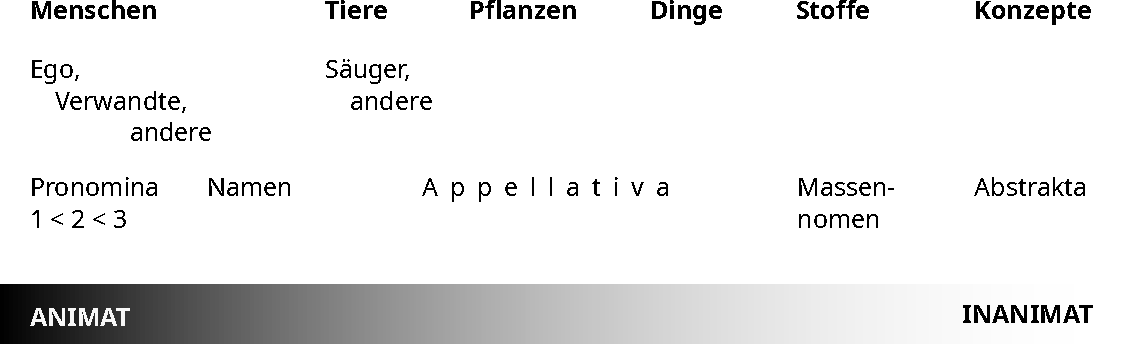
\includegraphics[
	width=\linewidth,
	keepaspectratio,
]{./figures/belebtheitshierarchie.pdf}
\caption{Belebtheitshierarchie \autocite[72]{kotthoffnuebling2018}}
\label{fig:animhier}
\end{figure}

Belebtheit wird als Kontinuum konzipiert; die Belebtheitshierarchie reicht von
Menschen als belebtester Kategorie über Tiere zu Gegenständen und Abstrakta als
am wenigsten belebt (siehe \figref{fig:animhier}). Die Sprecherinstanz steht
dabei gewöhnlich an der Spitze der Skala, da sie den Lokus der Wahrnehmung
bildet \autocites%
	{silverstein1976}%
	[185--200]{comrie1989}%
	[203]{bossong1998}%
	[40--46]{siewierska2004}%
	[439--441]{bickel2011}%
	[63--79]{kotthoffnuebling2018}. %
Belebtheit ist \citet[101--102, 110--112]{dahl1999} zufolge auch ein wichtiger
Faktor bei der Genuszuweisung, da ein hoher Grad von Belebtheit mit
semantischen Eigenschaften des Bezeichneten -- und hier gerade Sexus
beziehungsweise sexuelle Differenzierbarkeit -- als Quelle von Genus
korrelliert (\fw{referential gender}), während ein hoher Grad von Unbelebtheit
mit formalen Kriterien der Genuszuweisung einhergeht (\fw{lexical gender}). Wie
aus \figref{fig:animhier} deutlich wird, gibt es der Natur von Kontinua
entsprechend keine scharfe Grenze zwischen den Polen \emph{belebt} und
\emph{unbelebt}, sondern viele Übergangs- und Zweifelsfälle.

Da die Personen, die in den hier untersuchten Texten benannt werden, seit
Jahrhunderten tot und im Fall der \KC{} zusätzlich literarisch
überformt sind, lässt sich nicht nachvollziehen, wie sich das Verhältnis von
sozialem und biologischem Geschlecht in jedem einzelnen Fall genau verhält,
zumal es anachronistisch wäre, moderne Konzepte von sexueller Identität auf das
Hochmittelalter beziehungsweise die Antike im Spiegel eines
hochmittelalterlichen Texts zu übertragen \autocite[siehe
z.\,B.][]{klinger2002}. Weil Kontexte, in denen cis- und heterosexuelle Normen
explizit unterlaufen oder infrage gestellt werden, im Belegmaterial nicht
vorkommen, gehe ich bei der Klassifizierung meiner Daten von cis- und
heteronormativen Gegebenheiten aus.

Wenn im Weiteren vereinfachend von \textit{Sexus} als semantischer Basis von
Genus die Rede ist, bezieht sich der Begriff nicht primär auf eine biologische
Lesart. Vielmehr ist damit diejenige Geschlechter\-rolle gemeint, die in der
Wortbedeutung einer Personenbezeichnung angelegt ist und daher stereotyp
erwartet wird oder die vom Textzusammenhang etwa durch Namennennung implizierte
Geschlechterrolle. Gerade in der älteren Literatur ist in diesem Kontext häufig
vom \q{natürlichen Geschlecht} die Rede; \citet[67]{panther2009} spricht
diesbezüglich vom \q{konzeptuellen Genus}. Um auf das zuvor zitierte Beispiel
zurückzukommen, wird im Folgenden die Bezeichnung \fw{Mutter} entsprechend der
in der Wortbedeutung angelegten weiblichen Geschlechterrolle als eine weibliche
Person denotierend aufgefasst
\autocite[vgl.][s.\,v.~\fw{Mutter}]{duden-online}.

Bezüglich komplexer Kombinationen von Genus, Sexus und der Kongruenz darauf
bezogener Targets diskutiert \citet[183--184]{corbett1991} sogenannte
\fw{Lexical Hybrids}, also Substantive, deren Genus und Sexus nicht
übereinstimmen und bei denen in der pronominalen Referenz typischerweise
Variation zwischen formaler und semantischer Kongruenz herrscht, also zum
Beispiel, wenn \fw{das Mädchen} im weiteren Verlauf formal mit \fw{es} oder
semantisch mit \fw{sie} pronominal referenziert wird. \citet{klein2022}
unterscheidet darüber hinaus zwischen Lexical Hybrids im engeren Sinn und
Epikoina.

Bei Lexical Hybrids im engeren Sinn liegt ein Konflikt zwischen Genus und Sexus
auf der lexikalischen Ebene vor \autocite[145]{klein2022}. In diesem
Zusammenhang ist das historisch langlebige Wort für `Frau' als formales Neutrum
mit weiblicher Denotation hervorzuheben: Im Alt- und
Mittelhochdeutschen\il{Mittelhochdeutsch} lautet es \norm{wīb} beziehungsweise
\norm{wīp}. Auch im modernen Deutschen\il{Neuhochdeutsch} findet sich \fw{Weib}
noch mindestens bis ins 20.~Jahrhundert in nicht-pejorativer Verwendung
\autocite[166]{fleischer2012}. Im Fall von \fw{Mädchen} wird konventionell eine
junge weibliche Person bezeichnet, das neutrale Genus wird dem Lexem durch das
Diminutivsuffix \norm{-chen} formal zugewiesen. Auch bei Bezeichnungen wie
\fw{die Wache} oder, pejorativ, \fw{die Type} und \fw{die Tunte}, kommt es zu
Diskrepanzen in der Lexik, weil diese formal zu den Feminina zählen, jedoch in
ihrer Semantik gewöhnlich mit Männern assoziiert werden
\autocite[vgl.~auch][67--68]{panther2009}.

Eine andere Spielart von Lexical Hybrids liegt bei Epikoina vor, also im Grunde
sexus\-indifferenten Lexemen wie \fw{Person}, das zwar formal feminin ist, sich
aber der Wortbedeutung nach sowohl auf einen Menschen unabhängig von dessen
sozialem oder biologischem Geschlecht bezieht, oder \fw{Mensch}, das zwar
formal maskulin ist, für das aber prinzipiell dasselbe gilt.%
%
	\footnote{Siehe aber die Ergebnisse der Fragebogenstudie zu
		\fw{Mensch} und \fw{Person} von \citet[174--183]{klein2022}, bei denen
		die Probandinnen und Probanden in Einklang mit dem Genus des jeweiligen
		Lexems \norm{Mensch} eher mit Männern und \fw{Person} eher mit Frauen
		assoziiert haben.}
%
In diesen Fällen liegt in grammatisch spezifischen Kontexten ein Konflikt auf
der referenziellen Ebene vor, weil das jeweils geltende Sexusmerkmal von der
bezeichneten Person abhängt und damit vom konkreten Gebrauchskontext bestimmt
wird, also pragmatisch \autocite[142--144]{klein2022}.

Ein im Deutschen\il{Neuhochdeutsch} langlebiges Epikoinon ist \fw{Kind},
althochdeutsch\il{Althochdeutsch} \norm{kind} und
mittelhochdeutsch\il{Mittelhochdeutsch} \norm{kint}, das zwar formal neutral
ist, sich im konkreten Fall aber sowohl auf Mädchen als auch auf Jungen
beziehen kann, genereller auf nicht-erwachsene Menschen.%
%
	\footnote{Darüber hinaus kann sich \fw{Kind} im übertragenen Sinn auch auf
		erwachsene Menschen beziehen, zum Beispiel, wenn damit die
		Abhängigkeitsbeziehung zu den Eltern oder metaphorisch zu Gott betont
		wird \autocite[s.\,v.~\textit{kint}]{lexer:mhdhwb}. In manchen Fällen
		kann \fw{Kind} auch besonders auf Mädchen oder junge Frauen bezogen
		sein \autocites[808--816]{drw7}[s.\,v.~\textit{Kind}]{duden-online}.}
%
Insbesondere \fw{Kind} verdient Aufmerksamkeit, da die Variation zwischen
Neutrum in Einklang mit dem formalen Genusmerkmal sowie \emph{maskulin} oder
\fw{feminin} in Übereinstimmung mit dem semantischen Sexusmerkmal der
bezeichneten Person auch von deren Alter abhängt, insofern Kinder häufig als
weniger agentiv und damit weniger belebt als Erwachsene konzeptualisiert werden
\autocites[196]{comrie1989}[258--259]{birkenesfleischer2022}[151]{klein2022}.

In dieser Hinsicht stellt \citet[172--174]{klein2022} eine Hierarchie innerhalb
der Epikoina auf, da Abstufungen in der Belebtheit und, damit einhergehend, der
von Menschen wahrgenommenen Ausgeprägtheit sexueller Unterschiede zwischen
Individuen der bezeichneten Gruppe einen Einfluss darauf haben, ob ein
Epikoinon beim pronominalen Bezug eher mit formaler oder semantischer Kongruenz
steht \autocite[vgl.~auch][74--83]{kotthoffnuebling2018}. Sogenannte generische
Maskulina, also (vermeintlich) geschlechtsneutrale Bezeichnungen wie
\fw{Bürger} und \fw{Gast}, mittelhochdeutsch\il{Mittelhochdeutsch}
\norm{burgǟre} und \norm{gast}, bewegen sich darüber hinaus im Spannungsfeld
zwischen einer spezifischen, referenziellen Lesart mit Bezug auf einen
bestimmten Mann einerseits und einer unspezifischen, nicht-referenziellen
Lesart mit Bezug auf irgendein Individuum aus der benannten Gruppe und die
damit assoziierten stereotypen Geschlechterrollen andererseits
\autocites[91--122]{kotthoffnuebling2018}[159--160, 179--180]{klein2022}. Wo
zum Beispiel \norm{burgǟre} anders als in \REF{ex:nongenmasc} keine
spezifische Referenz besitzt, gehe ich im Folgenden vereinfachend davon aus,
dass damit allgemein die Stadt bewohnende Menschen gemeint sind.

\begin{exe}
\ex \label{ex:nongenmasc}
	\gll Hermann der Marſpurrer \textelp{} vnd Cvͦnrat der Turſte
			\textelp{} die {vor genemten} burgare bede von V́berlingen \\
		Hermann[\textsc{nom.sg.m}] der Marspurrer {} und
			Konrad[\textsc{nom.sg.m}] der Turste {} die vorgenannten
			Bürger[\textsc{nom.pl.m}] beid-\textsc{nom.pl.m} von Überlingen \\
	\trans `Hermann der Marspurrer \textelp{} und Konrad der Turste
		\textelp{}, die vorgenannten beiden Bürger von Überlingen' \\
		\parencites%
			(Nr.~N~288, Überlingen, Bodenseekr., 1285)%
			[223,19--21]{cao5}
\end{exe}

Körperteile stellen eine weitere Übergangskategorie dar, indem sie
Dingcharakter haben, aber Teil eines Organismus sind. Im speziellen Kontext mit
\norm{bėide} `beide' liegen in der Belegsammlung zu dieser Arbeit keine
Fälle von kombiniertem pronominalen Bezug auf Körperteile vor, sondern
lediglich der Fall in \REF{ex:bodyparts_attr}, bei dem \lit{baide}
`beide' attributiv \lit{hênde} `Hände' quantifiziert, sowie mehrere
Fälle mit \norm{bėide} als Konjunktion, von denen einer exemplarisch in
\REF{ex:bodyparts_conj} zitiert wird. In diesem Beispiel wird die Koordination
von \lit{ader} `Ader' und \lit{lit} `Glied' mit \lit{baidiv}
`beide' eingeführt, jedoch im weiteren Verlauf kein kombinierter Bezug auf
beide Konjunkte durch Pronomina hergestellt.

\begin{exe}
\ex \begin{xlist}
	\ex \label{ex:bodyparts_attr}
		\gll Si wand ír baide hênde \\
			sie wand ihr beid-\textsc{acc.pl.f.st} Hand-\textsc{acc.pl.f} \\
		\trans `Sie wand ihre beiden Hände.'
			(%
				K:~6rb,19; vgl. abweichend
				A1:~4va,26--27;
				H:~5va,4;
				M:~7vb,8;
				B1:~4vb,49;
				P:~9ra,5;
				\KC:~V.~913; \cite[98]{schroeder1895}% setno 1065
			)

	\ex \label{ex:bodyparts_conj}
		\gll baidiv ader unt lit. \\
			beide Ader[\textsc{acc.sg.f}] und Glied[\textsc{acc.sg.m/n}] \\
		\trans `sowohl Ader als auch Glied'
			(%
				A1:~32rb,31; vgl.
				H:~44va,15;
				M:~56vb,21;
				C1:~39rb,3;
				K:~45ra,32;
				Z:~147va,20;
				\KC:~V.~7468; \cite[218]{schroeder1895}% setno 2018
			)
\end{xlist}
\end{exe}

Der Belebtheitsstatus von Körperteilen ist zumindest im modernen
Standarddeutschen beachtenswert, da sich deren Possessivsyntax von anderen,
weniger belebten Dingen abhebt, wie die Beispiele in \REF{ex:stdgeralien}
zeigen. Dieses Verhalten lässt sich als Unterschied in der Alienabilität fassen
\autocites{nichols1988}[17--18]{heine1997}. Eine kursorische Suche im \REM{}
nach dem inalienablen Typ mit \textsc{pronomen}~(\textsc{dat}) --
\textsc{artikel}~(\textsc{acc}) -- \textsc{substantiv} hat keine Ergebnisse
geliefert.

	\begin{exe}
	\protectedex{%
	\ex \begin{xlist}
		\ex[]{Ich wasche mein Auto.
				\jambox{\hphantom{*\,}$\textsc{[+ alienabel]}$}}
		\ex[]{Ich wasche mir die Hände.
				\jambox{\hphantom{*\,}$\textsc{[- alienabel]}$}}
		\ex[*]{Ich wasche mir das Auto.
				\jambox{*\,$\textsc{[- alienabel]}$}}
		\end{xlist}
		\label{ex:stdgeralien}%
	}
	\end{exe}

Neben formalen und semantischen Merkmalen kann auch die Distanz zwischen einem
Controller und seinem Target einen Einfluss auf die Wahl der Kongruenzform
haben, wenn mehrere Möglichkeiten bestehen. Unter dieser Prämisse untersuchen
\citet{panther2009} und \citet{binanzeretal2022} semantische Kongruenz für die
moderne Standardsprache des Deutschen\il{Neuhochdeutsch}, \citet{fleischer2012}
geht diesem Aspekt in diachroner Perspektive nach. Diesen Studien ist die
Erkenntnis gemein, dass Kongruenz \fw{ad sensum} zum einen mit wachsender
linearer Distanz zwischen Controller und Target tendenziell zunimmt, zum
anderen verschiedene Arten von Pronomina und anaphorischen Ausdrücken eine
unterschiedlich hohe Affinität zur semantischen Kongruenz aufweisen, sich also
auch die syntaktische Domäne von Controller und Target auf die Wahl der
Kongruenzform auswirkt \autocites%
	(siehe auch \sectref{sec:ctrltarg}, \sectref{sec:kongrhier})%
	[84--85]{panther2009}[197--199]{fleischer2012}%
.

Da insgesamt also damit zu rechnen ist, dass die Semantik und der pragmatische
Kontext einer Personenbezeichnung einen starken Einfluss auf die Genuskongruenz
von anaphorischen Targets haben, möchte ich im Folgenden formale und
semantische Geschlechtsmerkmale in der Annotation von Beispielen konsequent
abbilden. Zu diesem Zweck erweitere ich die herkömmliche Annotation des Genus
um einen Index, der den Sexus kodiert, wie in \tabref{tab:gendsex} angegeben.

\begin{table}[h]
\centering
\caption{grammatisches und semantisches Geschlecht}
\begin{tabular}{l l l l} % @{\hspace{4\tabcolsep}}
\lsptoprule
\mc{2}{c}{Genus} & \mc{2}{c}{Sexus} \\ % \smallskip

\cmidrule(r){1-2}
\cmidrule(l){3-4}

\textsc{m} & maskulin & \SM & männlich     \\
\textsc{f} & feminin  & \SF & weiblich     \\
\textsc{n} & neutral  & \SI & unbelebt     \\
           &          & \SA & unspezifisch \\
           &          & \SX & unbekannt    \\
\lspbottomrule
\end{tabular}
\label{tab:gendsex}
\end{table}

Dabei wird für die Bezeichnung der formalen Kategorie \textit{Genus} die
lateinische Terminologie verwendet, für die Bezeichnung der semantischen
Kategorie \textit{Sexus} die deutsche. Zum Beispiel wird
\norm{wīp} `Frau' als \NeutF\ annotiert, \norm{kint} `Kind' je
nachdem, ob das Geschlecht des Kindes im Kontext bekannt ist, als \NeutM,
\NeutF\ oder \NeutX. Wenn sich im Kontext eines Beispiels \norm{ėrbe}
`Erbe' oder \norm{burgǟre} `Bürger' nicht auf eine bestimmte Person beziehen
lassen, also unspezifische Referenz vorliegt, werden sie mit \MascA\ annotiert.
Im Fall von \norm{schuech} `Schuh' als unbelebtem Substantiv steht \MascI, bei
\norm{minne} `Liebe' als Abstraktum \FemI. Da es sich bei Körperteilen nicht um
Menschen handelt, wurden auch diese unter Vorbehalt als Inanimata gewertet. So
wird \norm{hant} `Hand' mit \FemI{} annotiert, es sei denn, damit ist
metonymisch ein Diener oder eine Dienerin gemeint, in welchem Fall die
Annotation entsprechend \FemM{} oder \FemF{} lautet. Semantisch komplexe
Bezeichnungen wie \norm{drīvaltichėit} `Dreifaltigkeit' kommen im ausgewerteten
Material nicht vor. \norm{Got} `Gott' wurde gemäß seiner Bezeichnung als
\norm{truhtīn} `Herrscher' und \norm{hērre} `Herr' (z.\,B.\ \KC:~V.~8314, 13525;
\cite[234, 323]{schroeder1895}) als \MascM\ gewertet.

Im modernen Standarddeutschen liegen darüber hinaus einzelne Wörter wie
\fw{Schild} oder \fw{Korpus} vor, die je nach Bedeutungskontext
unterschiedliche Genera besitzen: \fw{das Schild} (\NeutI) für die
Hinweistafel, \fw{der Schild} (\MascI) für den Schläge und Hiebe abwehrenden
Schirm; \fw{der Korpus} (\MascI) als Schallkörper eines Saiteninstruments,
\fw{das Korpus} (\NeutI) als strukturierte Sammlung von Texten oder
Belegstellen. Ferner ist neben standardsprachlichem \fw{die Butter} (\FemI)
regional auch \fw{der Butter} (\MascI) verbreitet
\autocite[s.\,v.~\textit{der/die Butter}]{elspassmoeller2003}. Ein
mittelhochdeutsches\il{Mittelhochdeutsch} Beispiel für Substantive mit
bedeutungs\-unterscheidendem Genus ist \norm{dęr tėil} (\MascI) `Anteil,
Zugeteiltes, Eigentum' gegenüber \norm{daȥ tėil} (\NeutI) `Teil von einem
Ganzen, Stück, Seite, Abteilung' \autocite[s.\,v.~\textit{teil}]{lexer:mhdhwb}.

Des Weiteren liegt in der mittelhochdeutschen\il{Mittelhochdeutsch} Periode
noch eine größere Zahl an Substantiven vor, deren Genus bei gleicher Bedeutung
variabel belegt ist oder die ihr Genus im Lauf der Zeit gewechselt haben
\autocite[157--166]{ksw2}, zum Beispiel \norm{die} (\FemI) oder \norm{daȥ
jārƶīt} (\NeutI) `Jahrestag' sowie mittel\-hoch\-deutsch\il{Mittelhochdeutsch}
\fw{die wiƶƶe} (\FemI) `Wissen, Verstand, Klugheit'
\autocite[vgl.][s.\,v.~\textit{witze}]{lexer:mhdhwb} gegenüber
neu\-hoch\-deutsch\il{Neuhochdeutsch} \fw{der Witz} (\MascI). In diesen Fällen
wurde im Kontext der jeweiligen Text\-stelle nach Hinweisen gesucht, mit
welchem Genus das jeweilige Lexem verwendet wird, soweit dies möglich war.

\section{Gender Resolution}
\label{sec:gendres}

Ein Problem für Kongruenz entsteht dann, wenn zum Beispiel durch Koordination
von zwei Nominalen (Substantiven oder Personalpronomen) unterschiedliche
grammatische Merkmale derselben Kategorie (Genus, Numerus) pro Controller
vorliegen. Die Frage in diesem Fall ist, wie ein Target, das für die jeweilige
Kategorie flektiert, mit diesen divergierenden Merkmalen umgeht. Eine
Möglichkeit der Konfliktlösung besteht darin, lediglich mit dem nächsten
Konjunkt zu kongruieren \autocites[\fw{closest conjunct agreement};
vgl.][179--180]{corbett1983}[168--170]{corbett2006}, wie in dem Schema in
\figref{fig:ccagraphic} gezeigt.

\begin{figure}
\centering
\begin{tikzpicture}[
		baseline=(clbl.base),
		box/.style={
			draw,
			minimum height=2.5em,
		% 	font=\itshape,
		},
		wordbox/.style={
			draw,
			minimum height=1.75em,
		% 	font=\itshape,
		},
		lbl/.style={
			minimum height=1.5em,
			font={\smaller\scshape}
		},
		every node/.style={anchor=base}
	]

	\node [wordbox,                                ] (1) {A};
	\node [wordbox, base right=1ex of 1, draw=white] (2) {und};
	\node [wordbox, base right=1ex of 2            ] (3) {B};
	\node [         base right=3ex of 3            ] (4) {\dots};
	\node [wordbox, base right=3ex of 4, draw=white] (5) {C\tsub{B}};

	\node (C) [box, rectangle, fit={(1) (2) (3)}, thick] {};
	\node (T) [box, rectangle, fit=(5)                 ] {};

	\node (clbl) [lbl, above=.5ex of C] {controller};
	\node (tlbl) [lbl, above=.5ex of T] {target};

	\draw [-, draw=white, double=black, ultra thick] (3) -- ++(south:2em) -| (T);
	\node [lbl, below=1.25em of 4.south] {kongruenz};
\end{tikzpicture}

\begin{tikzpicture}[
		baseline=(clbl.base),
		box/.style={
			draw,
			minimum height=2.5em,
		% 	font=\itshape,
		},
		wordbox/.style={
			draw,
			minimum height=1.75em,
		% 	font=\itshape,
		},
		lbl/.style={
			minimum height=1.5em,
			font={\smaller\scshape}
		},
		every node/.style={anchor=base}
	]

	\node [wordbox,                                ] (1) {B};
	\node [wordbox, base right=1ex of 1, draw=white] (2) {und};
	\node [wordbox, base right=1ex of 2            ] (3) {A};
	\node [         base right=3ex of 3            ] (4) {\dots};
	\node [wordbox, base right=3ex of 4, draw=white] (5) {C\tsub{A}};

	\node (C) [box, rectangle, fit={(1) (2) (3)}, thick] {};
	\node (T) [box, rectangle, fit=(5)                 ] {};

	\node (clbl) [lbl, above=.5ex of C] {controller};
	\node (tlbl) [lbl, above=.5ex of T] {target};

	\draw [-, draw=white, double=black, ultra thick] (3) -- ++(south:2em) -| (T);
	\node [lbl, below=1.25em of 4.south] {kongruenz};
\end{tikzpicture}
\caption{Kongruenz mit dem nächsten Konjunkt}
\label{fig:ccagraphic}
\end{figure}

\citet[169]{corbett2006} gibt im Rahmen von Genuskongruenz das Beispiel in
\REF{ex:cca} aus dem Swahili\il{Swahili}. Dort treten \fw{kiti} `Stuhl' und
\fw{mguu wa meza} `Tischbein' auf, die jeweils einer unterschiedlichen
Nominalklasse angehören: \fw{kiti} `Stuhl' gehört zu den Klassen 7 (Sg.) und 8
(Pl.), \fw{mguu} `Bein' zu den Klassen 3 (Sg.) und 4 (Pl.). Das gemeinsame
Target \fw{u-/kimevunjika} zeigt Kongruenz in der Nominalklasse nur mit
demjenigen Konjunkt, das ihm am nächsten steht (3 bzw.~7).

\begin{exe}
\ex \label{ex:cca}
	\langinfo%
		{Swahili}%
		{}%
		{\cite[45]{bokamba1985} in \cite[169]{corbett2006}}
	\begin{xlist}
	\ex \label{ex:cca_1}
		\gll ki-ti na m-guu wa meza u-me-vunjika \\
			\textsc{cl7}-chair and \textsc{cl3}-leg of table
			\textsc{cl3}-\textsc{prf}-broken \\
		\trans `the chair and the leg of the table are broken'

	\ex \label{ex:cca_2}
		\gll m-guu wa meza na ki-ti ki-me-vunjika \\
			\textsc{cl3}-leg of table and \textsc{cl7}-chair
			\textsc{cl7}-\textsc{prf}-broken \\
		\trans `the leg of the table and the chair are broken'
	\end{xlist}
\end{exe}

In der Genuskongruenz der mittelhochdeutschen\il{Mittelhochdeutsch}
Sprachperiode wird in den oberdeutschen\il{Oberdeutsch} Schreibdialekten in
solchen Fällen die Kombinationsstrategie angewandt, wie in
\figref{fig:combgraphic} verdeutlicht
\autocites[vgl.][312]{grimm1890}[329]{grimm1898}[39--41]{behaghel1928}[187--189]{dal2014}:
Wenn für das Target keine Form der Deklinationsendung vorliegt, die im Plural
genusindifferent ist, muss der Unterschied zwischen den einzelnen Controllern
durch die Kombination ihrer Personenmerkmale aufgelöst werden, damit das Target
regelgemäß kongruieren kann
\autocites[vgl.][182--193]{corbett1983}[269--306]{corbett1991}[243--263]{corbett2006}.

\begin{figure}
\centering
\begin{tikzpicture}[
		baseline=(clbl.base),
		box/.style={
			draw,
			minimum height=2.5em,
		},
		wordbox/.style={
			draw,
			minimum height=1.75em,
		},
		lbl/.style={
			minimum height=1.5em,
			mynodefont,
		},
		every node/.style={anchor=base}
	]

	\node [wordbox,                                ] (1) {A};
	\node [wordbox, base right=1ex of 1, draw=white] (2) {und};
	\node [wordbox, base right=1ex of 2            ] (3) {B};
	\node [         base right=3ex of 3            ] (4) {\dots};
	\node [wordbox, base right=3ex of 4, draw=white] (5) {C\tsub{{A+B}}};

	\node (C) [box, rectangle, fit={(1) (2) (3)}, thick] {};
	\node (T) [box, rectangle, fit=(5)                 ] {};

	\node (clbl) [lbl, above=.5ex of C] {controller};
	\node (tlbl) [lbl, above=.5ex of T] {target};

	\draw [-, thick] (C) -- ++(south:2em) -| (T);
	\node [lbl, below=1em of $(2.south)!0.5!(5.south)$] {kongruenz};
\end{tikzpicture}
\caption{Kongruenz mit beiden Konjunkten}
\label{fig:combgraphic}
\end{figure}

Dies ist in den oberdeutschen\il{Oberdeutsch} Dialekten der Fall im Nom./Akk.\
Pl.\ der starken Adjektiv\-deklination \autocite[182]{ksw2}. Im Großteil der
ausgewerteten Belege steht daher aufgrund der Kombination der semantischen
Personenmerkmale die neutrale Form
\norm{bėidiu} `beide (\NeutMF)', wie in \REF{ex:gendres} in Bezug auf
\lit{Rvͦdiger} `Rüdiger (\MascM)' und seine \lit{hovſfrowe} `Ehefrau
(\FemF)' illustriert, auch wenn auf formaler Ebene \norm{bėide} `beide
(\textsc{m+f})' ansonsten sowohl für Maskulina als für auch Feminina gilt.

\begin{exe}
\ex \label{ex:gendres}
	\gll swenne aber her Rvͦdiger vnd ſin
			hovſfrowe bediv niht enſint\\
		so=wenn aber Herr Rüdiger[\textsc{nom.sg.\MascM}] und sein
			Ehefrau[\textsc{nom.sg.\FemF}] beide-\textsc{nom.pl.\NeutMF.st}
			nicht \textsc{neg}=sind \\
	\trans `Wenn aber Herr Rüdiger und seine Ehefrau beide
		nicht \textins{mehr} sind'
		\parencites%
			(Nr.~3262, Regensburg, 1299)%
			[425,13--14]{cao4}
\end{exe}

Eine direkte Entsprechung von \REF{ex:gendres} mit umgekehrter Reihenfolge der
grammatischen Merkmale der Konjunkte ist im ausgewerteten Material nicht
vorhanden, sondern lediglich der Fall mit \norm{bėide} als Modifikator
eines Personalpronomens, das sich seinerseits auf zwei Controller in dieser
Abfolge bezieht. \citet[96, 145]{askedal1973} führt die in
\REF{ex:askfmbeidiu} angeführten Stellen auf, die sich mit den leicht anders
formulierten Fällen im ausgewerteten Material decken, sodass davon auszugehen
ist, dass diese keine Sonderfälle darstellen. Da bei beiden Abfolgen von
\MascM\ und \FemF\ regelmäßig dieselbe Form \norm{bėidiu} auftritt, ist nicht
davon auszugehen, dass in \REF{ex:gendres} und \REF{ex:askfmbeidiu} Closest
Conjunct Agreement wie in \REF{ex:cca} auftritt und es sich bei \norm{bėidiu}
um eine Form des Nom.~Sg.~F.\ handelt, die ebenfalls auf \norm{-iu} endet.

\begin{exe}
	\ex \label{ex:askfmbeidiu}
		\begin{xlist}
		\ex \gll vnſer moͮter iwer frîundin. \\
				unser Mutter[\textsc{nom.sg.\FemF}] euer Freundin \\
		\sn \gll unde vnſer vater ſint beidiv tot. \\
				und unser Vater[\textsc{nom.sg.\MascM}] sind
				beide-\textsc{nom.pl.\NeutMF.st} tot \\
			\trans `Unsere Mutter, eure Freundin, und unser Vater sind beide
				tot.'
				(%
					\iai{Gottfried von Straßburg}, \tit{Tristan}: V.~18644--18645
					nach München, Bayerische Staatsbibl., Cgm~51: 96rb,23--24;
					% [\cite[1286]{hsc}];
					vgl.~\cite[259]{maroldschroeder1969}%
					% (= S. 259 → in ⁵2004: S. 313)
				)
			\label{ex:askfmbeidiu_1}
	
		\ex \gll {Condwir amvrſ} daz wip din \\
				Condwiramurs[\textsc{nom.sg.\FemF}] das Frau dein \\
		\sn \gll vn̄ din ſvn Loherangrin \\
				und dein Sohn[\textsc{nom.sg.\MascM}] Loherangrin \\
		\sn \gll sint beidiv mit dir dar benant \\
				sind beide-\textsc{nom.pl.\NeutMF} mit dir da benannt \\
		\trans `Condwiramurs, deine Frau, und dein Sohn Loherangrin
			sind beide mit dir dahin berufen.'
			(%
				\iai{Wolfram von Eschenbach}, \tit{Parzival}: 781,17--19
				nach St.~Gallen, Stiftsbibl., Cod.~Sang.~857: 275a,32--34;
				% [\cite[1211]{hsc}];
				vgl.~\cite[785]{knechtschirok2003}% (= S. 785)
			)
			\label{ex:askfmbeidiu_2}
	\end{xlist}
\end{exe}

\section{Kongruenz in der Lexical-Functional Grammar}
\label{sec:lfgkongr}

Die \fw{Lexical-Functional Grammar} (LFG;
\cites{kaplanbresnan1982,bresnan2001,bresnanetal2016}; \cites[zur Einführung
z.\,B.][]{buttking2015}[223--246]{mueller2023}) ist eine beschränkungsbasierte,
lexikalisch orientierte, nicht-trans\allowbreak{}formationale Grammatiktheorie
und basiert auf der Intuition, dass trotz aller Variation in der Syntax und
Morphologie die unterliegende funktionale Struktur (F-Struktur,
\fw{f-structure}) verschiedener Sprachen weitgehend gleich ist
\autocite[42]{bresnanetal2016}.
% %
% 	\footnote{\foreignblockcquote{english}[42]{bresnanetal2016}{The principle
% 		of universality states that \emph{internal structures are largely
% 		invariant across languages.} The formal model of internal structure in
% 		\textsc{lfg} is the f-structure, which stands for \q{functional
% 		structure}}.%
% 	}
% %
Die sprachliche Grundlage, auf der die LFG entwickelt wurde und
weiterentwickelt wird, ist typologisch sehr breit aufgestellt.
\citet[223--224]{mueller2023} gibt einen exemplarischen Überblick über die
Sprachen, für die mehr oder weniger ausführliche Beschreibungen in diesem
Theorieframework vorliegen \autocites[zum modernen Standarddeutschen
vgl.][]{berman2003}{fortmann2006}. Die Wahl der theoretischen Anbindung ist der
Praktikabilität geschuldet. Die LFG operiert vornehmlich mit grammatischen
Merkmalen im Sinne \posscite{corbett2012} im Zusammenspiel mit der
Konstituentenstruktur und ist damit bestens geeignet, um Kongruenz als
morphosyntaktisches Phänomen zu analysieren.
% ; der Annotationsformalismus und die
% Darstellung von Merkmalsstrukturen sind vergleichsweise unkompliziert.

Hauptbestandteil des Formalismus der LFG ist die funktionale Struktur
(F-Struktur), die eine der als parallel gedachten Repräsentationsebenen
darstellt, auf denen Sprache operiert \autocite[840--844]{buttking2015}.%
%
	\footnote{\citet[862--865]{buttking2015} nennen darüber hinaus zum Beispiel
		noch die
		A-Struktur (Argumente),
		I-Struktur (Information),
		M-Struktur (Morphologie),
		P-Struktur (Prosodie)
		und die
		S-Struktur (Semantik).
	}
%
Die F-Struktur wird in Attribut-Wert-Matrizen dargestellt (\fw{attribute-value
matrices}; \cites[vgl.][44--45]{bresnanetal2016}[207--221]{mueller2023}), die
Informationen strukturiert präsentieren, vergleiche \figref{fig:avm}. Als
Attribute in der linken Spalte dienen Funktionen oder Merkmale wie Subjekt
(\textsc{subj}), Objekt (\textsc{obj}), Prädikator (\textsc{pred}) oder
Numerus (\textsc{num}). Zugehörige Werte in der rechten Spalte können
grammatische Eigenschaften wie Plural (\textsc{pl}), Funktionsmorpheme wie
\textit{und}, Wortformen wie `Baum', A-Strukturen wie
\astruct{schreiben}{\ups{subj}, \ups{obj}} sowie F-Strukturen oder Mengen von
F-Struk\-turen sein. Jedem Attribut sind dabei ein oder mehrere eindeutige
Werte zugewiesen; Funktionen (\textsc{subj}, \textsc{obj}, etc.) können nur
einfach instanziiert werden \autocite[vgl.][44--58]{bresnanetal2016}.

\begin{figure}
\centering
	{% \avmsetup{attributes=\scshape}
	\avm{[
		vorname		& `Max' \\
		nachname	& `Meier' \\
		geburtstag	& 10.\,10.\,1985 \\
		vater		& [
			vorname		& `Peter' \\
			nachname	& `Meier' \\
			geburtstag	& 10.\,5.\,1960 \\
			vater		& \dots \\
			mutter		& \dots \\
		] \\
		mutter		& \dots \\
	]}}
\caption{Attribut-Wert-Matrix \autocite[nach][209]{mueller2023}}
\label{fig:avm}
\end{figure}

Darüber hinaus wird eine Konstituentenstruktur (\fw{constituent structure},
\fw{c-struc\-ture}) angesetzt, die parallel zur F-Struktur den Aufbau von
syntaktischen Konstituenten abbildet und eine Variante der \xbar{X}-Theorie
\autocites{chomsky1970,jackendoff1977} darstellt. Projektionen innerhalb des
Baumes können dabei funktional annotiert sein; nicht-verzweigende
\xbar{X}-Kategorien werden als überflüssig angesehen und in der Regel
weggelassen, wie in \figref{fig:cfstruct}, wo kein struktureller Unterschied
zwischen Spezifikator, Adjunkt und Komplement gemacht wird, weil die Annotation
disambiguiert.

\begin{figure}
\begin{forest} align text
[CP\mysn{cfstruct_CP}
	[{\anno[\pass{subj}]{NP\mysn{cfstruct_NP}}}
	 	[\anno{\xhead{N}\mysn{cfstruct_N}}
	 		[Lola]
	 	]
	]
	[\anno{\xhead{C}\mysn{cfstruct_C}}
		[rennt]
	]
]
\node [avmcontainer] {\avm{%
	\tikzmark{cfstruct_f}$f$: [
		pred	& \astruct{rennen}{\ups{subj}} \\
		tense	& \textsc{prs} \\
		%
		subj	&	\tikzmark{cfstruct_subj}$g$: [
			pred	& `Lola' \\
			pers	& 3 \\
			num		& \textsc{sg} \\
			case	& \textsc{nom} \\
		]
	]%
}}; 
\end{forest}
\begin{tikzpicture}[remember picture, overlay]
	\draw [myarrow]
		([yshift=.5ex]{pic cs:cfstruct_CP})
		to [out=east, in=west]
		([yshift=.5ex]{pic cs:cfstruct_f});
	\draw [myarrow]
		([yshift=.5ex]{pic cs:cfstruct_C})
		to [out=east, in=west]
		([yshift=.5ex]{pic cs:cfstruct_f});
	\draw [myarrow]
		({pic cs:cfstruct_NP})
		to [out=south east, in=west]
		([yshift=.5ex]{pic cs:cfstruct_subj});
	\draw [myarrow]
		([yshift=.5ex]{pic cs:cfstruct_N})
		to [out=east, in=west]
		([yshift=.5ex]{pic cs:cfstruct_subj});
\end{tikzpicture}
\caption{Analyse des Satzes \fw{Lola rennt}}
\label{fig:cfstruct}
\end{figure}

In \figref{fig:cfstruct} wird die Korrespondenz zwischen der C-Struktur und der
F-Struktur des Satzes \fw{Lola rennt} dargestellt. Der Satz betsteht aus einer
NP mit dem Kopf \fw{Lola}, die das Subjekt (\textsc{subj}) des Satzes
darstellt, und einer Komplementiererphrase (\fw{complementizer phrase}, CP),
die das Subjekt dominiert und das (flektierte) Verb \fw{rennt} zum Kopf hat.
Ein Pfeil nach unten (↓) bezeichnet in der Annotation den jeweiligen Knoten
selbst, ein Pfeil nach oben (↑) den darüber liegenden. \q{\pass{subj}} ist
daher so zu verstehen, dass die Informationen in dem damit annotierten Knoten
die Eigenschaften der Subjekt\-funk\-tion des darüberliegenden Knotens
darstellen. Die optionalen Pfeile zwischen C- und F-Struktur verdeutlichen,
welcher Knoten seine Informationen in welcher F-Struktur (hier: $f$ oder $g$)
ablegt. Die F-Struktur wird vom Verb \fw{rennen} prädiziert (\textsc{pred}) und
nimmt als Argument ein Subjekt \ups{subj}. Dessen grammatische Eigenschaften
bilden den Wert des Attributs Subjekt (\textsc{subj}).

Dabei wird ein wichtiges Merkmal der LFG sichtbar: Informationen des jeweiligen
Knotens werden mit dem nächsthöheren Knoten vereinigt. Das bedeutet, dass
Attributen stets eindeutige und miteinander kompatible Werte zugewiesen sein
müssen, um einen kohärenten Ausdruck zu erzeugen
\autocite[vgl.][43--54]{bresnanetal2016}. Anders als im eingangs vorgestellten
morphologischen Ansatz entsteht Kongruenz hier durch den Abgleich von
grammatischen Merkmalen. \citet[7]{wechslerzlatic2003} zufolge wird Kongruenz
also nicht als gerichteter Prozess verstanden, bei dem Merkmalsbündel kopiert
oder verschoben werden, sondern als das Zusammenspiel zweier Elemente, die
partielle Informationen über dasselbe linguistische Objekt spezifizieren.
Kongruenz resultiert daraus, dass die von den beiden Quellen gebotenen
Informationen kompatibel miteinander sein müssen.
% %
% 	\footnote{\foreignblockcquote{english}[7]{wechslerzlatic2003}{%
% 		\textins*{A}greement is not viewed as a directional process of copying
% 		or moving feature bundles, but rather as two elements specifying
% 		partial information about a single linguistic object. Agreement results
% 		from the fact that this information coming from two sources must be
% 		compatible}.
% 	}
% %
Dies wird in \figref{fig:lolamorphlex} verdeutlicht, wo die Lexikoneinträge für
\fw{Lola} und \fw{rennt} vereinfacht wiedergegeben werden.

\begin{figure}
\begin{tabular}[t]{@{} l @{\hspace{2em}} c @{\hspace{2em}} l}
	$Lola$
	&	N
	&	\begin{tabular}[t]{l l l}
			\ups{pred}	& =	& `Lola' \\
			\ups{pers}	& =	& 3 \\
			\ups{num}	& =	& \textsc{sg} \\
		\end{tabular}
	\medskip \\

	$rennt$
	&	C
	&	\begin{tabular}[t]{l l l}
			\ups{pred}		& = 	& \astruct{rennen}{\ups{subj}} \\
			\ups{subj pers}	& \req	& 3 \\
			\ups{subj num}	& \req	& \textsc{sg} \\
		\end{tabular}
\end{tabular}
\caption{Morpholexikalische Definition von \fw{Lola} und \fw{rennt}}
\label{fig:lolamorphlex}
\end{figure}

\fw{Lola} bildet als Substantiv einen Diskursanker und definiert (=) die
angegebenen Merk\-male: 3.~Person und Singular. Die finite Verbform \fw{rennt}
bedingt (\req) ihrem Lexikoneintrag gemäß eine Subjekt-NP, die die
Personenmerkmale 3.~Person und Singular aufweist. Da die Personenmerkmale von
\fw{Lola} diese Bedingung (\fw{constraint}) erfüllen, kommt es zur Kongruenz
zwischen Subjekt und Verb
\autocite[vgl.][59]{bresnanetal2016}.

In Anlehnung an die Beispiele \REF{ex:coordidx} und \REF{ex:engartdiscong} in
\figref{fig:lfgcoord_1} und \ref{fig:lfgcoord_2} noch einmal zur Illustration
die jeweils grammatisch akzeptablen Varianten vor dem Hintergrund des gewählten
Theorieframeworks gezeigt. Die Annotation der koordinierten NPs folgt
\citet{peterson2004}. In \figref{fig:lfgcoord_1} erfordert das Verb
\fw{spielen} ein Subjekt mit den Personenmerkmalen 3.~Person und Plural in
Übereinstimmung mit dem kombinierten Index der Subjekt-NP in $g$; zwei
Singulare ergeben zusammen einen Plural.%
%
	\footnote{Mit \q{g-und} wird das gruppenbildende \fw{und} bezeichnet, bei
		dem sich die Konjunkte auf jeweils unterschiedliche Indizes $i, j$
		beziehen \autocite[382--383]{dalrymple2001}.}

\begin{figure}
\begin{forest} shorter edges, narrower nodes, align text
[CP\mysn{lfgcoord1_CP}
	[{\anno[\pass{subj}]{NP\mysn{lfgcoord1_NP1}}}
		[{\anno[\updownelem]{\xhead{N}}}
			[Jan]
		]
		[Conj
			[und]
		]
		[{\anno[\updownelem]{\xhead{N}}}
			[Markus]
		]
	]
	[\anno{\xbar{C}}
		[\anno{\xhead{C}}
			[spielen, name=spielen, minimum width=4em]
		]
		[\anno{VP\mysn{lfgcoord1_VP}}
			[{\anno[\pass{obj}]{NP\mysn{lfgcoord1_NP2}}}
				[\anno{\xhead{N}}
					[Fußball]
				]
			]
		]
	]
]
%
% Annotation des Knotens zu breit, als dass die AVM noch hinpasst
\node at (spielen) [below=1ex] {
	\smaller[2]\upshape\tabcolsep=.5ex%
	\begin{tabular}[t]{@{} l l l @{}}
		\ups{subj pers}	& \req & 3 \\
		\ups{subj num}	& \req & \textsc{pl} \\
	\end{tabular}%
};
%
\node [avmcontainer=1em, font=\footnotesize] {
	\avm{%
	\tikzmark{lfgcoord1_f}$f$: [
		pred	& \astruct{spielen}{\ups{subj}, \ups{obj}} \\
		tense	& \textsc{prs} \\
		%
		subj	& \tikzmark{lfgcoord1_g}$g$: [
			conj & \textit{g-und} \\
			%	
			\mc{2}{l}{%
				\{
					[
						pred	&	`Jan' \\
						index	&	[
							pers	& 3 \\
							gend	& \textsc{m} \\
							num		& \textsc{sg} % \\
						] \\
						case	& \textsc{nom} % \\
					]\smallskip\\
					%
					[
						pred	&	`Markus' \\
						index	&	[
							pers	& 3 \\
							gend	& \textsc{m} \\
							num		& \textsc{sg} % \\
						] \\
						case	& \textsc{nom} % \\
					]
				\}%
			} \\
			%
			index	&	[
				pers	& 3 \\
				num		& \textsc{pl} \\
			] \\
		] \\
		%
		obj	& \tikzmark{lfgcoord1_h}$h$: [
			\normalfont{\q{Fußball}}
		] \\
	]}
};
\end{forest}
\begin{tikzpicture}[remember picture, overlay]
	\draw [myarrow]
		([yshift=.5ex]{pic cs:lfgcoord1_CP})
		-- ++(right:1.5em)
		to [out=east, in=west]
		([yshift=.5ex]{pic cs:lfgcoord1_f});
	\draw [myarrow]
		([yshift=.5ex]{pic cs:lfgcoord1_VP})
		to [out=east, in=west, min distance=0.5cm]
		([yshift=.5ex]{pic cs:lfgcoord1_f});
	\draw [myarrow]
		([yshift=.5ex]{pic cs:lfgcoord1_NP1})
		to [out=east, in=north west]
		([yshift=.5ex]{pic cs:lfgcoord1_g});
	\draw [myarrow]
		([yshift=.5ex]{pic cs:lfgcoord1_NP2})
		to [out=east, in=north west]
		([yshift=.5ex]{pic cs:lfgcoord1_h});
\end{tikzpicture}
\caption{Analyse des Satzes \fw{Jan und Markus spielen Fußball}}
\label{fig:lfgcoord_1}
\end{figure}

Demgegenüber ist es innerhalb der in \figref{fig:lfgcoord_2} gezeigten NP
notwendig, dass der De\-termi\-nierer \fw{diese} im Numerus mit dem
Concord-Merkmal jedes einzelnen der beiden Konjunkte übereinstimmt, damit
Kongruenz hergestellt werden kann und ein kohärenter, grammatisch wohlgeformter
Ausdruck entsteht.%
%
	\footnote{Im Deutschen\il{Neuhochdeutsch} kommen noch Kasus und Genus
	hinzu, die hier vereinfachend weggelassen wurden. \citet{dalrymple2001}
	benutzt \emph{Spezifikator} (\textsc{spec}) als grammatische Funktion bei
	der Annotation des Determinierers, \citet{bresnanetal2016} hingegen
	behandeln \emph{Spezifikator} als Merkmal. Beide folgen in ihren Beispielen
	der DP-Hypothese \autocite{chomsky1986}, für die sich u.\,a.\ auch
	\citet[9--26]{demske2001} ausspricht, insofern sie sie als sinnvoll für die
	Analyse von NPs im Deutschen\il{Neuhochdeutsch} erachtet.}
%
\citet[91--94]{kingdalrymple2004} zufolge stellen Modifikatoren im
Deutschen\il{Neuhochdeutsch} zusätzlich Bedingungen an Index-Merkmale.

\begin{figure}
	\begin{forest} narrower nodes, align text
	[{\anno[\pass{subj}]{DP\mysn{lfgcoord2_DP}}}
		[\anno{\xhead{D}}
			[diese, name=diese, minimum width=4em]
		]
		[{\anno{NP\mysn{lfgcoord2_NP}}}
		% 	[\anno{\xbar{N}}
				[{\anno[\updownelem]{\xhead{N}}}
					[Jungen]
				]
				[Conj
					[und]
				]
				[{\anno[\updownelem]{\xhead{N}}}
					[Mädchen]
				]
		% 	]
		]
	]
	%
	% Annotation des Knotens zu breit, als dass die AVM noch hinpasst
	\node at (diese) [below=1ex] {
		\smaller[2]\upshape\tabcolsep=.5ex%
		\begin{tabular}[t]{@{} l l l @{}}
			\ups{concord num}	& \req & \textsc{pl} \\
			\ups{index num}		& \req & \textsc{pl} \\
		\end{tabular}%
	};
	%
	\node [avmcontainer, font=\footnotesize] {
		\avm{%
		\tikzmark{lfgcoord2_f}$f$: [
			spec	& [
				pred	& `diese'
			] \\
			%
			conj	& \textit{g-und} \\
			%
			\mc{2}{l}{%
				\{
					[
						pred	& `Jungen' \\
						%
						concord	& [
							case	& \textsc{nom} \\
							num		& \textsc{pl} \\
							gend	& \textsc{m}
						] \\
						%
						index	& [
							pers	& 3 \\
							num		& \textsc{pl} \\
							gend	& \textsc{m}
						]
					]\smallskip\\
					%
					[
						pred	& `Mädchen' \\
						%
						concord	& [
							case	& \textsc{nom} \\
							num		& \textsc{pl} \\
							gend	& \textsc{f}
						] \\
						%
						index	& [
							pers	& 3 \\
							num		& \textsc{pl} \\
							gend	& \textsc{f}
						]
					]
				\}%
			} \smallskip \\
			%
			index	& [
				pers	& 3 \\
				num		& \textsc{pl} \\
			]
		]}
	};
	\end{forest}
	\begin{tikzpicture}[remember picture, overlay]
		\draw [myarrow]
			([yshift=.5ex]{pic cs:lfgcoord2_NP})
			to [out=east, in=west]
			([yshift=.5ex]{pic cs:lfgcoord2_f});
		\draw [myarrow]
			([yshift=.5ex]{pic cs:lfgcoord2_DP})
			-- ++(right:1em)
			to [out=east, in=west]
			([yshift=.5ex]{pic cs:lfgcoord2_f});
		% \draw [myarrow]
		% 	([yshift=.5ex]{pic cs:lfgcoord2_DP})
		% 	to [out=east, in=west]
		% 	([yshift=.5ex]{pic cs:lfgcoord2_g});
	\end{tikzpicture}
\caption{Analyse des Satzfragments \fw{diese Jungen und Mädchen}}
\label{fig:lfgcoord_2}
\end{figure}

Da der Plural im modernen Deutschen\il{Neuhochdeutsch} keine
Genusdifferenzierung aufweist, ist der Ausdruck im Beispiel möglich. Wenn die
Konjunkte im Singular stehen, können die unterschiedlichen Genus-Merkmale
jedoch nicht vereinigt werden: *\fw{dieser/s Junge und Mädchen}.

Die unterschiedlichen syntaktischen Domänen nach \citet[54]{corbett2006}, die
in \sectref{sec:ctrltarg} vorgestellt wurden, lassen sich in der Terminologie
der LFG als Abhängigkeiten zwischen immer weniger lokalen F-Strukturen fassen,
insofern (lexikalische) C-Strukturköpfe (\xhead{X}) mit F-Strukturköpfen
(Prädikatoren, \textsc{pred}) korrespondieren \autocite[117]{bresnanetal2016}.
Dies wird anhand von \figref{fig:fstructdomains} verdeutlicht.

Dort ist \fw{braune} als adjektivisches Kongruenztarget ein Adjunkt von
\fw{Katze} und steht damit in derselben F-Struktur $g$ wie sein Controller
(gleiche NP). Auf \fw{Katze} ist ebenfalls der Possessor \fw{Janas} in $h$
bezogen. \fw{Janas} und \fw{Katze} befinden sich zwar in verschiedenen
F-Strukturen ($g$ und $h$), allerdings ist der Possessor in $h$ Teil der
Subjektfunktion $g$ (gleicher Satzteil). Das Reflexivpronomen \fw{sich} in $j$
bildet das direkte Objekt von \fw{putzen}. Da es sich bei dem Objekt um ein
Reflexivpronomen handelt, ist es mit dem Subjekt in $g$ koindiziert und stellt
ebenfalls dessen Kongruenztarget dar, allerdings steht \fw{sich} als Objekt in
einer anderen F-Struktur als das Subjekt ($j$ gegenüber $g$). Da aber Subjekt
und Objekt vom gleichen Verb \fw{putzen} abhängen, befinden sich beide dennoch
innerhalb derselben F-Struktur $f$ (gleicher Satz).

\begin{figure}
	\begin{forest} shorter edges, narrower nodes, align text
	[CP\mysn{fsdom_CP}
		[{\anno[\pass{subj}]{DP\mysn{fsdom_DPs}}}
			[{\anno[\pass{poss}]{DP\mysn{fsdom_DPp}}}
				[\anno{\xhead{D}}
					[Janas]
				]
			]
			[\anno{NP\mysn{fsdom_NP}}
				[{\anno[\elem{adj}]{AP\mysn{fsdom_AP}}}
					[\anno{\xhead{A}}
						[braune]
					]
				]
				[\anno{\xhead{N}}
					[Katze]
				]
			]
		]
		[\anno{\xbar{C}}
			[\anno{\xhead{C}}
				[putzt]
			]
			[\anno{VP\mysn{fsdom_VP}}
				[{\anno[\pass{obj}]{DP\mysn{fsdom_DPr}}}
					[\anno{\xhead{D}}
						[sich]
					]
				]
			]
		]
	]
	%
	\node [avmcontainer=2ex, font=\footnotesize] {
		\avm{%
			\tikzmark{fsdom_f}$f$: [
				subj	& \tikzmark{fsdom_subj}$g$: [
					poss	& \tikzmark{fsdom_poss}$h$: [
						pred	& `Jana' \\
						case	& \textsc{gen} \\
					] \\
					%
					adj		& \tikzmark{fsdom_adj}\{
						[
							pred	& `braun'
						]
					\} \\
					%
					pred	& \astruct{Katze}{\ups{poss}} \\
					case	& \textsc{nom} \\
					pers	& 3 \\
					gend	& \textsc{f} \\
					num		& \textsc{sg} \\
				]~$i$ \\
				%
				pred	& \astruct{putzen}{\ups{subj}, \ups{obj}} \smallskip \\
				%
				obj	& \tikzmark{fsdom_obj}$j$: [
					prontype	& $refl$ \\
					pred		& $pro$ \\
					case		& \textsc{acc} \\
				]~$i$ \\
			]}
	};
	\end{forest}
	\begin{tikzpicture}[remember picture, overlay]
		\draw [myarrow]
			([yshift=.5ex]{pic cs:fsdom_CP})
			-- ++(right:1em)
			to [out=east, in=west]
			([yshift=.5ex]{pic cs:fsdom_f});
		\draw [myarrow]
			([yshift=.5ex]{pic cs:fsdom_VP})
			to [out=east, in=west]
			([yshift=.5ex]{pic cs:fsdom_f});
		\draw [myarrow]
			([yshift=.5ex]{pic cs:fsdom_DPs})
			to [out=east, in=west]
			([yshift=.5ex]{pic cs:fsdom_subj});
		\draw [myarrow]
			([yshift=.5ex]{pic cs:fsdom_DPp})
			to [out=east, in=west]
			([yshift=.5ex]{pic cs:fsdom_poss});
		\draw [myarrow]
			([yshift=.5ex]{pic cs:fsdom_AP})
			to [out=east, in=west]
			([yshift=.5ex]{pic cs:fsdom_adj});
		\draw [myarrow]
			([yshift=.5ex]{pic cs:fsdom_DPr})
			to [out=east, in=west]
			([yshift=.5ex]{pic cs:fsdom_obj});
	\end{tikzpicture}
	\caption{Analyse des Satzes \fw{Janas braune Katze putzt sich}}
	\label{fig:fstructdomains}
\end{figure}

\section{Floating Quantifiers}
\label{sec:floatquant}

Wenn im Rahmen dieser Arbeit der Terminus \textit{Quantor} verwendet wird, dann
werden darunter solche Determinierer eines nominalen Ausdrucks verstanden, die
etwas über seine Anzahl oder Menge aussagen, wie zum Beispiel \fw{alle, manche,
einige} oder auch \fw{beide}. Dabei ist zu beachten, dass sich verschiedene
Quantoren syntaktisch unterschiedlich verhalten
\autocites[27--28]{pittner1995}[11--12]{haspelmath1997}. Das in dieser Arbeit
insbesondere behandelte \fw{beide} bezeichnet eine Menge von genau zwei
im Kontext eindeutig identifizierbaren Elementen einer Gruppe
\autocite[vgl.][307]{keenan2006} und ist damit definit
\autocite[265--268]{lyons1999}.

Als Modifikatoren von Substantiven (und in manchen Fällen auch Pronomen, zum
Beispiel \fw{sie beide}, \fw{alle diese}) unterliegen Quantoren wie
\norm{bėide} im Mittelhochdeutschen\il{Mittelhochdeutsch} wie auch \fw{beide}
im Neuhochdeutschen\il{Neuhochdeutsch} der Adjektivdeklination. Das bedeutet,
sie kongruieren mit ihrem nominalen Controller formal in den Kategorien Kasus
(\textsc{case}), Genus (\textsc{gend}) und Numerus (\textsc{num}) über ein
fusionales Suffix, das diese Eigenschaften kombiniert kodiert
\autocites(vgl.~auch \sectref{sec:ctrltarg},
\sectref{sec:lfgkongr})[181--184]{ksw2}[772]{woellstein2022}. Daneben ist bei
\fw{beide} im Deutschen\il{Neuhochdeutsch} zu beachten, dass es zusammen mit
einem Definit- oder Possessivartikel auftreten kann \REF{ex:beidedet_2}, anders
als Definit- und Possessivartikel selbst, die gewöhnlich in komplementärer
Distribution zu einander stehen (*\fw{das mein Buch}). Im Unterschied zu
Adjektiven ist es andererseits aber auch nicht möglich, in der syntaktischen
Position von \fw{beide} weitere Wörter vom gleichen Typ unterzubringen, weder
durch Koordination \REF{ex:beidedet_3} noch durch Reihung
\REF{ex:beidedet_4}, wie es etwa bei Adjektiven trotz Restriktionen
bezüglich ihrer Abfolge grundsätzlich möglich ist. Im Unterschied zu Adjektiven
können Quantoren vom Typ \fw{alle} und \fw{beide} im
Deutschen\il{Neuhochdeutsch} außerdem nicht prädikativ gebraucht werden, wie
aus \REF{ex:beidepred_2} deutlich wird (vgl.~auch \cite[181,
Fußnote~1]{merchant1996}).

\begin{exe}
\label{ex:beidedet}
\ex \begin{xlist}
	\ex[]{beide/wenige Bücher}
		\label{ex:beidedet_1}
	\ex[]{die beiden/wenigen Bücher}
		\label{ex:beidedet_2}
	\ex[*]{die beiden und wenigen Bücher}
		\label{ex:beidedet_3}
	\ex[*]{die beiden, wenigen Bücher}
		\label{ex:beidedet_4}
\end{xlist}

\ex \begin{xlist}
	\ex glückliche/beide/viele Hunde
		\label{ex:beidepred_1}
	\ex Die Hunde sind glücklich/*beide/\tsup{?}viele.
		\label{ex:beidepred_2}
\end{xlist}
\end{exe}

Aufgrund dieser Unterschiede sowohl zu \q{typischen} Determinierern als auch zu
Adjektiven wird in Einklang mit der im folgenden zu besprechenden Literatur
angenommen, dass Quantoren wie \fw{beide} eine gesonderte funktionale Kategorie
\xhead{Q} nominalen Typs repräsentieren. Anders als zum Beispiel
\fw{all} und das englische\il{Englisch} \fw{both} `beide', die ganz links in
der Nominalgruppe stehen (\fw{all die \dots}, \fw{both the \dots}), reiht sich
die Quantorenphrase (QP) mit \fw{beide} im Standarddeutschen gewöhnlich
zwischen DP und NP ein, wie in \figref{fig:nomstack} dargestellt (vgl.~auch
\cite[44--45 mit Fußnote 30]{lyons1999}). Als funktionale nominale Kategorie
ist \xhead{Q} wie \xhead{D} aus Sicht der LFG ein Ko-Kopf von \xhead{N}
(\fw{cohead}; \cite[124]{bresnanetal2016}). Dies bedeutet, dass die Information
in DP und QP mit NP in derselben F-Struktur vereinigt wird. Zusätzlich wird
hier angenommen, dass der Quantor zumindest bei seiner Verwendung innerhalb der
DP der Quantor als Merkmal (\textsc{quant}) definiert, da er aufgrund des
distributiven Unterschieds zu Adjektiven nicht als Teil der Menge der Adjunkte
(\textsc{adj}) gezählt werden sollte.

\begin{figure}
	\begin{forest} narrower nodes, align text
	[DP\mysn{nomstack_DP}
		[\anno{\xhead{D}}
			[die]
		]
		[\anno{QP\mysn{nomstack_QP}}
			[\anno{\xhead{Q}}
				[beiden]
			]
			[\anno{NP\mysn{nomstack_NP}}
				[{\anno[\elem{adj}]{AP}}
					[roten]
				]
				[\anno{\xhead{N}}
					[Bücher]
				]
			]
		]
	]
	%
	\node [avmcontainer] {
		\avm{%
		\tikzmark{nomstack_f}[
			def	& $+$ \\
			%
			quant	& 	[
				pred	& `beide' \\
			] \\
			%
			adj	& \{
				[
					pred	& `rot'
				]
			\} \\
			%
			pred	& `Buch' \\
			case	& \textsc{nom} \\
			pers	& 3 \\
			gend	& \textsc{n} \\
			num		& \textsc{pl} \\
		]}
	};
	\end{forest}
	\begin{tikzpicture}[remember picture, overlay]
		\draw [myarrow]
			([yshift=.5ex]{pic cs:nomstack_DP})
			to [out=east, in=west]
			([yshift=.5ex]{pic cs:nomstack_f});
		\draw [myarrow]
			([yshift=.5ex]{pic cs:nomstack_QP})
			to [out=east, in=west]
			([yshift=.5ex]{pic cs:nomstack_f});
		\draw [myarrow]
			([yshift=.5ex]{pic cs:nomstack_NP})
			to [out=east, in=west]
			([yshift=.5ex]{pic cs:nomstack_f});
	\end{tikzpicture}
	\caption{Analyse des Satzfragments \fw{die beiden roten Bücher}}
	\label{fig:nomstack}
\end{figure}

\citet[790]{schwartz2000} hebt darüber hinaus hervor, dass Quantoren wie
\fw{jeder}, \fw{manche} und \fw{alle} auch eine pronominale Funktion ausüben
können \autocite[vgl.~auch][11--12]{haspelmath1997}. In diesen Fällen steht der
Quantor nicht attributiv zu einem Substantiv wie in \figref{fig:nomstack}, sondern
fungiert als eigenständiger Kopf eines Satzglieds \REF{ex:quantpron}.

\begin{exe}
\ex \label{ex:quantpron}
\begin{xlist}
	\ex \parbox[t]{.55\linewidth}{%
			Anna\tsub{i} liest gerne und Paul\tsub{j} auch.\\
			Beiden\tsub{{i+j}} habe ich ein Buch geschenkt.%
		}\jambox{(indirektes Objekt)}
		\label{ex:quantpron_1}
	\ex \parbox[t]{.55\linewidth}{%
			Ich brauche einen neuen Mixer\tsub{i}.\\
			Er\tsub{i}/Dieser\tsub{i}/Meiner\tsub{i} ist kaputt.%
		}\jambox{(Subjekt)}
		\label{ex:quantpron_2}
\end{xlist}
\end{exe}

In \REF{ex:quantpron_1} bezieht sich \fw{beiden} auf \fw{Anna} und \fw{Paul},
steht jedoch in einem anderen Satz. Während \norm{Anna und Paul} das Subjekt
von \norm{lesen} bilden, stellt \fw{beiden} das indirekte Objekt von
\fw{geschenkt} dar. Dabei ist zu beachten, dass \fw{beiden} einen bestimmten
Bezugskontext benötigt. Das Paar, das der Quantor referenziert, muss also durch
den sprachlichen Kontext eindeutig identifizierbar sein
\autocites[vgl.~z.\,B.][274]{lyons1999}[788]{schwartz2000}[983]{janssen2004}.
Genauso verhalten sich die Pronomina \fw{er} (Personalpronomen), \fw{dieser}
(Demonstrativpronomen) und \fw{meiner} (Possessivpronomen) in
\REF{ex:quantpron_2}, insofern auch sie definit sind und voraussetzen, dass
ein eindeutiger Bezug hergestellt werden kann
\autocites[vgl.][145--148]{lyons1999}. Dieser wird im Beispiel durch den
\fw{Mixer} im vorangehenden Satz gegeben.

Ein weiteres Charakteristikum von Quantoren wie \fw{alle},
\fw{beide}, \fw{einige} oder \fw{viele} ist, dass sie innerhalb desselben
Satzes getrennt von ihrer Nominalgruppe stehen können, wie in
\REF{ex:floatsubj} mit Bezug auf das Subjekt gezeigt. Die Versionen mit
Distanzstellung in (b) und (c) sind jeweils markiert, insofern der Fokus auf
der Menge liegt. Allerdings müssen auch hier mehrere, oberflächlich ähnliche
Konstruktionen unterschieden werden
\autocites[27--28]{pittner1995}[65--67]{fanselowcavar2002}.

\begin{exe}
\ex \label{ex:floatsubj}
\begin{xlist}
	\ex \label{ex:floatsubj_1}
		{\ob}\tsub{QP}~Alle {\ob}\tsub{NP}~Kinder{\cb}{\cb} mögen Schokolade.
	\ex \label{ex:floatsubj_2}
		{\ob}\tsub{DP}~Die Kinder{\cb}\tsub{i} mögen {\ob}\tsub{QP}~alle{\cb}\tsub{i}
		Schokolade.
	\ex \label{ex:floatsubj_3}
		{\ob}\tsub{QP}~Alle{\cb}\tsub{i} mögen {\ob}\tsub{DP}~sie/*die
		Kinder{\cb}\tsub{i} Schokolade.
\end{xlist}
\end{exe}

\citet{sportiche1988} beschäftigt sich mit der Syntax des Allquantors \fw{tous}
`alle' im Französischen\il{Französisch}. Er argumentiert, dass Quantoren, die
getrennt von ihrer Bezugs-NP rechts vom Verb stehen, keine Adverbien sind, wie
zuvor vorgeschlagen wurde, sondern in einem anaphorischen Verhältnis zu der NP
stehen, die sie modifizieren \autocite[428--433]{sportiche1988}. Ferner werde
nicht der Quantor nach rechts verschoben (\q{gefloatet}), sondern die
Subjekt-NP aus ihrer Position hinter dem Quantor aus der Verbphrase extrahiert,
also nach vorn gezogen. Dabei werde eine Spur (\fw{trace}; t) zurückgelassen,
was die anaphorische Relation zwischen Quantor und Quantifiziertem erkläre
\autocite[432--433]{sportiche1988}. Eigentlich handelt es sich also um
Stranding -- das Zurücklassen von syntaktischem Material an der Stelle seiner
ursprünglichen Generierung.

\citet{shlonsky1991} untersucht dies am modernen Hebräischen (\ili{Ivrit}) und
bestätigt weitgehend \citeauthor{sportiche1988}s Erkenntnisse. Aufgrund der
Daten aus dem \ili{Ivrit} modifiziert er \posscite{sportiche1988} Hypothese
über die Konstituenz der Konstruktion dahingehend, dass Quantor und
Quantifiziertes eine Quantorenphrase mit dem Quantor als Kopf und einer
Determiniererphrase (DP) als Komplement bilden. \citet{merchant1996} überträgt
die Erkenntnisse von \citet{sportiche1988} und \citet{shlonsky1991} auf das
Deutsche\il{Neuhochdeutsch} und nimmt weitere Verfeinerungen ihrer Hypothese
bezüglich möglicher Positionen des gestrandeten Quantors vor. Für das
Englische\il{Englisch} \fw{all} `alle' mit Bezug auf das Subjekt gibt
\citet{merchant1996} grob die Konstituentenstruktur in \figref{fig:qfgg} an
(die Pfeile wurden zur Verdeutlichung der postulierten Transformation
hinzugefügt).

\begin{figure}
	\begin{forest} shorter edges
	[IP
		[DP\tsub{i}
			[{the boys},roof,name=DP]
		]
		[\xbar{I}
			[\xhead{I}
				[have]
			]
			[VP
				[QP
					[t′\tsub{i},name=t2]
					[\xbar{Q}
						[\xhead{Q}
							[all]
						]
						[t\tsub{i},name=t1]
					]
				]
				[\xbar{V}
					[\xhead{V}
						[seen]
					]
					[DP
						[{the film},roof]
					]
				]
			]
		]
	]
	\draw [-latex, gray] (t1) to [out=west, in=south] (t2);
	\draw [-latex, gray] (t2) to [out=west, in=south] (DP);
	\end{forest}
	\caption{Analyse des Satzes \fw{The boys have all seen the film}
	\autocite[nach][180]{merchant1996}}
	\label{fig:qfgg}
\end{figure}

\citet{sportiche1988}, \citet{shlonsky1991} und \citet{merchant1996}
beschränken sich sämtlich auf den Quantor \fw{alle}, nur \citet{pittner1995}
geht darüber hinaus und untersucht auch das ähnlich funktionierende \fw{beide};
nur diese beiden fasst sie im Rahmen ähnlicher Konstruktionen als \q{gefloatete
Quantoren} auf. Was darüber hinaus \citeauthor{shlonsky1991},
\citeauthor{pittner1995} und \citeauthor{merchant1996} eint, ist, dass sie alle
den Unterschied in der Lesart zwischen der Version mit Kontaktstellung und der
mit Distanzstellung behandeln. Der Unterschied wird in
\figref{fig:siebeidefhrd_1} und \ref{fig:siebeidefhrd_2} den Beispielen bei
\citet[30--31]{pittner1995} folgend illustriert.

\begin{figure}
\begin{tikzpicture}[baseline=(A.base)]
	\node [draw, rectangle] (A) at (0,1) {A};
	\node [draw, rectangle] (B) at (2,1) {B};
	\node [draw, rectangle] (fhrd1) at (0,0) {Fahrrad};
	\node [draw, rectangle] (fhrd2) at (2,0) {Fahrrad};
	\draw [-latex] (A) -- (fhrd1);
	\draw [-latex] (B) -- (fhrd2);
\end{tikzpicture}
\\
\caption{Sie haben beide ein Fahrrad}
\label{fig:siebeidefhrd_1}
\end{figure}

\begin{figure}
\begin{tikzpicture}[baseline=(A.base)]
	\node [draw, rectangle] (A) at (0,1) {A};
	\node [draw, rectangle] (B) at (4,1) {B};
	\node [draw, rectangle, gray] (fhrd1) at (0,0) {Fahrrad};
	\node [draw, rectangle      ] (fhrd)  at (2,0) {Fahrrad};
	\node [draw, rectangle, gray] (fhrd2) at (4,0) {Fahrrad};
	\draw [-latex] (A) to [out=east, in=north] (fhrd);
	\draw [-latex] (B) to [out=west, in=north] (fhrd);
	\draw [-latex, gray] (A) -- (fhrd1);
	\draw [-latex, gray] (B) -- (fhrd2);
\end{tikzpicture}
\caption{Sie beide haben ein Fahrrad}
\label{fig:siebeidefhrd_2}
\end{figure}

Während der Satz in \figref{fig:siebeidefhrd_1} mit gefloatetem Quantor
ausschließlich die Lesart zulässt, bei der beide Parteien jeweils ein Fahrrad
besitzen (distributive Lesart), lässt das Beispiel in \figref{fig:siebeidefhrd_2}
zusätzlich die Interpretation zu, nach der beide Parteien gemeinsam ein Fahrrad
besitzen (kollektive Lesart). Zusätzliche Betonung des Quantors kann in diesem
Fall zwar zur Disambiguierung beitragen (\emph{Sie \emph{beide} haben ein
Fahrrad} = distributiv), ist aber bei der rein textlichen Wiedergabe von Sprache
ohne spezielle Markierung nicht nachvollziehbar.

\phantomsection
\label{phsec:hebrqf}
Die bisher referierten Artikel diskutieren Floating Quantifiers im Rahmen von
Government and Binding \autocite{chomsky1981}. Wie könnte eine Adaption in die
LFG aussehen? Diesen Versuch unternimmt \citet{spector2009} in Rückgriff auf
\citet{shlonsky1991} für das \ili{Ivrit}, siehe \REF{ex:hebrqf} und
\figref{fig:hebrqf}. Anders als im Deutschen\il{Neuhochdeutsch} oder im
Französischen\il{Französisch} kongruiert der gefloatete Quantor (\fw{kol}
`alle') dort nicht bloß, sondern beinhaltet ein klitisches Pronomen, das mit
dem Quantifizierten koindiziert ist.%
%
	\footnote{Im Sinne der Grammatikalisierungs\-theorie nach
		\citet{lehmann2015} stellt Klitisierung eine Vorstufe von Kongruenz dar
		\autocite[vgl.][44]{lehmann2015}.%
	}

\begin{exe}
\ex \label{ex:hebrqf}
	\langinfo%
		{Ivrit}
		{}
		{\cite[nach][522, 537]{spector2009}}\\
	\gll ha-yeladim halxu kulam la-yam \\
		\textsc{def}=children[\textsc{3pl.m}]\tsub{i} went all=\textsc{3pl.m}\tsub{i}
			to=sea.\textsc{def} \\
	\trans `The children went all to the sea.'
\end{exe}

\begin{figure}
	\begin{forest} shorter edges, narrower nodes, align text
	[IP\mysn{hebrqf_IP}
		[NP\mysn{hebrqf_NP}
			[\xhead{N}
				[ha-yeladim]
			]
		]
		[\xbar{I}
			[\xhead{I}
				[halxu]
			]
			[S%\mysn{hebrqf_S}
				[QP\mysn{hebrqf_QP}
					% [\xbar{Q}
						[\xhead{Q}
							[kulam]
						]
					% ]
				]
				[VP%\mysn{hebrqf_VP}
					[PP\mysn{hebrqf_PP}
						[la-yam, roof]
					]
				]
			]
		]
	]
	%
	\node [avmcontainer, font=\footnotesize] {
		\avm{\tikzmark{hebrqf_f}[
			top	& \tikzmark{hebrqf_top}[
				pred	& `child' \\
				def		& $+$ \\
				num		& \textsc{pl} \\
			]~$i$
			\smallskip \\
			%
			subj	& \tikzmark{hebrqf_subj}[
				pred	& \astruct{all}{\ups{obj}} \\
				obj	& [
					pred	& $pro$ \\
					pers	& 3 \\
					gend	& \textsc{m} \\
					num		& \textsc{pl} \\
				]~$i$ \\
			]
			\smallskip \\
			%
			pred	& \astruct{went}{\ups{subj}, \ups{\Oblq{dir}}}
			\smallskip \\
			%
			\Oblq{dir}	& \tikzmark{hebrqf_obl}[
				pred	& \astruct{to}{\ups{obj}} \\
				obj	& [
					pred	& `sea' \\
					def		& $+$ \\
					num		& \textsc{sg} \\
				] \\
			] \\
		]}
	};
	\end{forest}
	\begin{tikzpicture}[remember picture, overlay]
		\draw [myarrow]
			([yshift=.5ex]{pic cs:hebrqf_IP})
				to [out=east, in=west]
			([yshift=.5ex]{pic cs:hebrqf_f});
		% \draw [myarrow]
		% 	([yshift=.5ex]{pic cs:hebrqf_S})
		% 		to [out=east, in=west]
		% 	([yshift=.5ex]{pic cs:hebrqf_f});
		% \draw [myarrow]
		% 	([yshift=.5ex]{pic cs:hebrqf_VP})
		% 		to [out=east, in=west]
		% 	([yshift=.5ex]{pic cs:hebrqf_f});
		%
		\draw [myarrow]
			([yshift=.5ex]{pic cs:hebrqf_NP})
				to [out=east, in=west]
			([yshift=.5ex]{pic cs:hebrqf_top});
		\draw [myarrow]
			([yshift=.5ex]{pic cs:hebrqf_QP})
				to [out=east, in=west]
			([yshift=.5ex]{pic cs:hebrqf_subj});
		%
		\draw [myarrow]
			([yshift=.5ex]{pic cs:hebrqf_PP})
				to [out=east, in=west]
			([yshift=.5ex]{pic cs:hebrqf_obl});
	\end{tikzpicture}
	\caption{Analyse des Satzes \fw{Ha-yeladim halxu kulam la-yam} `Die Kinder
		fuhren alle ans Meer'}
		% \foreignlanguage{hebrew}{הילדים הלכו כולם לים}
	\label{fig:hebrqf}
\end{figure}

\citet[533--534]{spector2009} kommt ähnlich wie \citet[29]{pittner1995} zu dem
Schluss, dass der gefloatete Quantor eine eigenständige NP darstellt. Die
Topikalisierung des Quantifizierten werde durch die Distanzstellung des
Quantors angezeigt; die Konstruktion sei dadurch besonders markiert. Beide NPs,
Topik (\textsc{top}) und Subjekt (\textsc{subj}), sind in
\citeauthor{spector2009}s Analyse durch Koindizierung verbunden, werden aber
nicht in der F-Struktur miteinander vereinigt
\autocite[vgl.][99]{bresnanetal2016}.

Die Analysen von \citet{shlonsky1991} und \citet{spector2009} für das
\ili{Ivrit} könnten insofern für die Analyse des Deutschen\il{Neuhochdeutsch}
relevant sein, als \citet[179]{merchant1996} eine Ähnlichkeit zwischen dem
hebräischen\il{Ivrit} \fw{kol} `alle' und dem deutschen\il{Neuhochdeutsch}
\fw{alle} bezüglich des Auftretens von Flexion in Abhängigkeit der
Stellungsvariante vermerkt: Die Kongruenzendung fehlt, wenn der Quantor einer
definiten NP vorangeht: \fw{all die X} aber \fw{alle X}. Der Fall von \fw{die
beiden X} und \fw{beide X} würde eine separate Diskussion benötigen.
Nachfolgend möchte ich einige vorläufige Überlegungen zur Modellierung der
Situation im Mittelhochdeutschen\il{Mittelhochdeutsch} anstellen.

Während im modernen Standarddeutschen Determinierer und Adjektive normalerweise
links vom Substantiv stehen, können Adjektive im
Mittelhochdeutschen\il{Mittelhochdeutsch} auch rechts davon auftreten
\autocite[185--186, 237--243]{ksw2}, selten auch Determinierer wie
Possessivartikel, \norm{dehėin} `kein' und \norm{bėide}
\autocite[515--517, 551--552, 623--624]{ksw2}. Im hier ausgewerteten Material
liegen immerhin zwanzig Fälle im \tit{Corpus der altdeutschen Originalurkunden}
(\CAO) und drei in der \tit{Kaiserchronik} (\KC) mit nachgestelltem
\norm{bėide} hinter einem einfachen Plural-Substantiv vor
\REF{ex:beidepost_2}.


\begin{exe}
	\ex \label{ex:beidepost_2}
		\gll ſo man die iargezit beidú begat \\
			so man die Jahrestag[\textsc{acc.pl.\NeutI}]
			beide-\textsc{acc.pl.\NeutI.st} begeht \\
		\trans `wenn man die Jahrestage beide begeht'
			\parencites%
				(Nr.~3331, Straßburg und Colmar, 1299)%
				[468,21--22]{cao4}
\end{exe}

Da die LFG ohne Transformationen auskommt (also keine Verschiebungen von
syntaktischen Einheiten auf einer abstrakten Ebene wie in \figref{fig:qfgg}
angenommen werden), bietet sich für die Lesart mit Kontaktstellung in
\figref{fig:beidepost_2cont} an, \norm{die} (\xhead{D}) und \norm{bėide}
(\xhead{Q}) als funktionale Ko-Köpfe von \norm{jārƶīt} `Jahrestag' (\xhead{N})
zu behandeln.%
%
	\footnote{Artikel und Quantor sind im ursprünglichen Beispiel nicht
		kongruent, insofern \norm{jārƶīt} entweder feminin oder neutral belegt
		ist \autocite[s.\,v.~\fw{jârzît}]{lexer:mhdhwb}. Der Artikel \norm{die}
		flektiert maskulin-feminin, der Quantor \norm{bėidiu} dagegen neutral.
		Neutrum in Bezug auf einen unbelebten Referenten lässt sich als
		semantische Kongruenz interpretieren, was die Lesart in
		\figref{fig:beidepost_2dist} mit pronominal verwendetem \norm{bėidiu}
		plausibler macht.}

\begin{figure}
	\begin{forest} shorter edges, narrower nodes, align text
	[VP
		[{\anno[\pass{obj}]{DP\mysn{beidepost2c_DP}}}
			[\anno{\xhead{D}}
				[die]
			]
			[\anno{QP\mysn{beidepost2c_QP}}
				[\anno{NP\mysn{beidepost2c_NP}}
					[\anno{\xhead{N}}
						[jārƶīt]
					]
				]
				[\anno{\xhead{Q}}
					[bėide]
				]
			]
		]
		[\anno{\xhead{V}}
			[begāt]
		]
	]
	%
	\node [avmcontainer] {
		\avm{%
		\tikzmark{beidepost2c_f}$f$: [
			obj	& \tikzmark{beidepost2c_obj}[
				def	& $+$ \\
				pred	& `Jahrestag' \\
				case	& \textsc{acc} \\
				num		& \textsc{pl} \\
				gend	& \textsc{f} \\
				anim	& $-$ \\
				quant	& [
					pred	& `beide' \\
				] \\
			] \\
			%
			pred	& \astruct{begehen}{\ups{subj}, \ups{obj}} \\
		]}
	};
	\end{forest}
	\begin{tikzpicture}[remember picture, overlay]
	\draw [myarrow]
		([yshift=.5ex]{pic cs:beidepost2c_NP})
		to [out=east, in=south west]
		([yshift=.5ex]{pic cs:beidepost2c_obj});
	\draw [myarrow]
		([yshift=.5ex]{pic cs:beidepost2c_QP})
		to [out=east, in=south west]
		([yshift=.5ex]{pic cs:beidepost2c_obj});
	\draw [myarrow]
		([yshift=.5ex]{pic cs:beidepost2c_DP})
		to [out=east, in=south west]
		([yshift=.5ex]{pic cs:beidepost2c_obj});
	\end{tikzpicture}
	\caption{Analyse des Satzfragments \norm{die jārƶīt bėide begāt} `die beiden Jahrestage begeht'}
	\label{fig:beidepost_2cont}
\end{figure}

Basierend auf der Analyse von \citet{spector2009} für das \ili{Ivrit} dient das
Schema in \figref{fig:beidepost_2dist} als Arbeits\-hypothese für die Lesart
mit gefloatetem Quantor. Parallel zu Subjekt (\textsc{subj}) und Topik
(\textsc{top}) werden hier die Rollen Objekt (\textsc{obj}) und Fokus
(\textsc{foc}) für \norm{bėidiu} und die dazugehörige DP angenommen. Die
aufeinander bezogenen Teile ($g$ und $h$) sind koindiziert ($i$), um die
anaphorische Funktion von \norm{bėide} zu erfassen.%
%
	\footnote{Die Annotationsform \q{\uncertain{$x$}{$a$}~\req~$v$} in
		\figref{fig:beidepost_2dist} bedeutet, dass entsprechend der Flexion der
		annotierten Wortform außerhalb des lokalen Funktionskerns (hier $h$)
		eine grammatische Funktion $x$ als Controller existiert, die ein
		Attribut $a$ besitzt, das den Wert $v$ für sein Target voraussetzt
		(\fw{inside-out functional uncertainty};
		\cite[66--70]{bresnanetal2016}).}
%
Eine eingehendere Diskussion der Konstruktion müsste auf die Bindungsrelation,
etwa im Vergleich zu Reflexivpronomina, und gegebenenfalls funktionale
Präzedenz eingehen \autocite[vgl.][213, 254--285]{bresnanetal2016}. Auch für
den in \REF{ex:floatsubj_3} illustrierten Unterschied in der Akzeptabilität
von \textit{Alle mögen sie/*die Kinder Schokolade} könnte dies eine Rolle
spielen.

\begin{figure}
	\begin{forest}
		shorter edges,
		narrower nodes,
		align text
	[VP
		[\anno{VP}
			[{\anno[\pass{foc}]{DP\mysn{beidepost2d_DP}}}
				[\anno{\xhead{D}}
					[die]
				]
				[\anno{NP\mysn{beidepost2d_NP}}
					[\anno{\xhead{N}}
						[jārƶīt]
					]
				]
			]
			[\anno{VP}
				[{\anno[\pass{obj}]{QP\mysn{beidepost2d_QP}}}
					[\anno{\xhead{Q}}
						[bėidiu, name=beidiu, minimum width=5em]
					]
				]
			]
		]
		[\anno{\xhead{V}}
			[begāt]
		]
	]
	%
	% Annotation des Knotens zu breit, als dass die AVM noch hinpasst
	\node at (beidiu) [below=1ex] {
		\smaller[2]\upshape\tabcolsep=.5ex%
		\begin{tabular}[t]{@{} l l l @{}}
			\uncertain{$x$}{case}	& \req & \textsc{acc} \\
			\uncertain{$x$}{num}	& \req & \textsc{pl} \\
			\uncertain{$x$}{gend}	& \req & \textsc{n} \\
			$\lor$ \uncertain{$x$}{anim} & \req & $-$ \\
		\end{tabular}%
	};
	%
	\node [avmcontainer] {
		\avm{%
		\tikzmark{beidepost2d_f}$f$: [
			foc	& \tikzmark{beidepost2d_foc}$g$: [
				def		& $+$ \\
				pred	& `Jahrestag' \\
				case	& \textsc{acc} \\
				num		& \textsc{pl} \\
				gend	& \textsc{f} \\
				anim	& $-$ \\
			]~$i$ \smallskip \\
			%
			obj	& \tikzmark{beidepost2d_obj}$h$: [
				pred	& `beide' \\
			]~$i$ \\
			%
			pred	& \astruct{begehen}{\ups{subj}, \ups{obj}} \\
		]}
	};
	\end{forest}
	\begin{tikzpicture}[remember picture, overlay]
	\draw [myarrow]
		([yshift=.5ex]{pic cs:beidepost2d_NP})
		to [out=east, in=west]
		([yshift=.5ex]{pic cs:beidepost2d_foc});
	\draw [myarrow]
		([yshift=.5ex]{pic cs:beidepost2d_QP})
		to [out=east, in=west]
		([yshift=.5ex]{pic cs:beidepost2d_obj});
	\draw [myarrow]
		([yshift=.5ex]{pic cs:beidepost2d_DP})
		to [out=east, in=west]
		([yshift=.5ex]{pic cs:beidepost2d_foc});
	\end{tikzpicture}
	\caption{Analyse des Satzframents \norm{die jārƶīt bėidiu begāt} `die
		Jahrestage beide begeht'}
	\label{fig:beidepost_2dist}
\end{figure}

Die Schemata in \figref{fig:beidepost_2cont} und \ref{fig:beidepost_2dist}
zeigen außerdem, dass die Nachstellung des Quantors tendenziell zu
syntaktischer Ambiguität führt. In den hier gesammelten Daten tritt das Problem
vor allem bei den zahlreichen Belegen für \norm{si bėide} auf, wenn \norm{si}
im Mittelfeld steht (vgl.~\figref{fig:sibeideambig}). Kontaktstellung ist also
nicht gleich Kontaktstellung, da auch in Kontaktstellung ein gefloateter
Quantor vorliegen kann. \citet[623--624]{ksw2} benennen dieses Problem
ebenfalls und zählen \blockquote{solche Fälle immer als attributiv
nachgestellt}, also wie in \figref{fig:sibeideambig} rechts dargestellt.

\begin{figure}
\begin{forest}
	shorter edges,
	align text,
	[\anno{VP}
		[{\anno[\pass{gf}]{QP}}
			[\anno{DP}
				[\anno{\xhead{D}}
					[si]
				]
			]
			[\anno{\xhead{Q}}
				[bėide]
			]
		]
		[\anno{\xbar{V}}
			[\dots]
		]
	]
\end{forest}
\hspace{2em}
\begin{forest}
	shorter edges,
	align text,
	[\anno{VP}
		[{\anno[\pass{df}]{DP}}
			[\anno{\xhead{D}}
				[si]
			]
		]
		[\anno{VP}
			[{\anno[\pass{gf}]{QP}}
				[\anno{\xhead{Q}}
					[bėide]
				]
			]
			[\anno{\xbar{V}}
				[\dots]
			]
		]
	]
\end{forest}
\caption{Zwei Varianten von oberflächlicher Kontaktstellung}
\label{fig:sibeideambig}
\end{figure}

\section{Die Kongruenzhierarchie}
\label{sec:kongrhier}

Die von \citet{corbett1979} formulierte Kongruenzhierarchie (\fw{agreement
hierarchy}) basiert auf dem typologischen Vergleich einer Reihe
(indo-)europäischer Sprachen, die sowohl formale als auch semantische Kongruenz
zulassen.%
%
	\footnote{Dies sind: 
		Deutsch, % \il{Neuhochdeutsch},
		Englisch, % \il{Englisch},
		Französisch, % \il{Französisch},
		Lateinisch, % \il{Lateinisch},
		Russisch und % \il{Russisch},
		Spanisch % \il{Spanisch}
	\autocite[214--215]{corbett1979}. Die Stichprobe ist durch die Beschränkung
	auf große europäische Sprachen typologisch nicht repräsentativ.
	\citet[218]{corbett2006} listet weitere Sprachen auf -- auch
	nicht-indogermanische --, für die seitdem Untersuchungen durchgeführt
	wurden.}
%
Das Ergebnis der Studie ist, dass mit wachsender \q{syntaktischer Distanz}
zwischen Controller und Target die Wahrscheinlichkeit für das Auftreten von
semantischer statt formaler Kongruenz steigt \autocite[218--223]{corbett1979}.
\citet[204]{corbett1979} formuliert die Kongruenzhierarchie folgendermaßen:

\begin{exe}
\ex attributive > predicate > relative pronoun > personal pronoun
\end{exe}

Je weiter links ein Target einzuordnen ist, desto höher ist die
Wahrscheinlichkeit, dass formale Kongruenz auftritt; je weiter rechts, desto
höher die Wahrscheinlichkeit für semantische Kongruenz. Die Abfolge ist
monoton: Wenn bei einem Targettyp semantische Kongruenz möglich ist, ist dies
auch bei allen Targettypen rechts von ihm möglich. Da für das
Deutsche\il{Neuhochdeutsch} manche von \citeauthor{corbett1979}s Kategorien für
den von ihm untersuchten Genusausgleich relevanter als andere sind (Genus ist
kein Merkmal der Verbalflexion; Possessivpronomen kongruieren doppelt), schlägt
\citet[193]{fleischer2012} mit einem Blick speziell auf die Genus-Kongruenz
folgende Konkretisierung vor:

\begin{exe}
\ex Artikel, attributives Demonstrativpronomen \\
	\hspace*{1em} > andere attributive Relationen \\
	\hspace*{2em} > Relativpronomen \\
	\hspace*{3em} > anaphorisches Demonstrativpronomen, Personalpronomen \\
	\hspace*{4em} > anaphorisches Possessivpronomen
\end{exe}

Er betont den Sonderstatus des Relativpronomens, das sowohl eine anaphorische
als auch eine attributive Funktion hat, und merkt weiterhin an, dass das
\blockcquote[194]{fleischer2012}{attributiv verwendete Adjektiv und Partizip
\textelp{} im Spätalthochdeutschen\il{Althochdeutsch} und
Mittelhochdeutschen\il{Mittelhochdeutsch} auch mit semantischer Kongruenz
auf\textins{tritt}, umgekehrt zeigt das Personalpronomen in älteren
althochdeutschen\il{Althochdeutsch} und vor allem in den jüngsten
neuhochdeutschen\il{Neuhochdeutsch} Texten auch formale Kongruenz}.

Bezogen auf die syntaktische Motivation der empirisch erarbeiteten Erkenntnisse
schreibt \citet[216]{corbett1979}, dass attributive Kongruenz auf die einfache
Phrase beschränkt sei, prädikative Kongruenz die Phrase überschreite doch auf
den Teilsatz beschränkt bleibe, während Personalpronomen nicht auf den Satz der
Instanz beschränkt sei, die die Kongruenzbeziehung kontrolliert.
% %
% 	\footnote{\foreignblockcquote{english}[216]{corbett1979}{%
% 		\textins*{A}ttributive agreement represents agreement within the simple
% 		phrase, predicative agreement goes beyond the phrase but is restricted
% 		to the clause, the agreement of the relative pronoun goes beyond the
% 		clause but is restricted to the sentence, while the personal pronoun is
% 		not restricted to the sentence of the item controlling agreement}.}

Die Kernthese von \citet{wechslerzlatic2003} ist daher, dass formale Kongruenz
bei Attributen zu erwarten ist, da innerhalb der NP Concord das entscheidende
Kongruenzmerkmal darstellt. Hingegen ist semantische Kongruenz bei
Personalpronomen außerhalb der bindenden NP deshalb mit höherer
Wahrscheinlichkeit zu erwarten, weil Pronomen über den referenziellen Index an
ihren Referenten gebunden sind \autocite[89--91]{wechslerzlatic2003}. Die
Autoren argumentieren also für eine Korrelation zwischen der Distribution von
Kongruenz zeigenden Wortarten, deren syntaktischer Lokalität sowie den
anwendbaren Kongruenz\-merkmalen.

\citet[89]{wechslerzlatic2003} erklären weiter, dass Personalpronomen auch
deiktisch oder exophorisch verwendet werden können, also mit Verweis auf
außersprachliche Referenten, ohne dass diese zunächst innersprachlich verankert
wurden. In diesen Fällen komme entweder grammatische oder pragmatische
Kongruenz zum Zuge, letztere speist sich aus der Semantik des Bezeichneten.
Relativpronomina seien dagegen immer anaphorisch gebunden -- wobei sich die
Autoren hier vermutlich auf den innersprachlichen Kontext beziehen -- und
kongruieren in Index-Merkmalen, möglicherweise auch in Concord-Merkmalen, da
sie NP-intern auftreten. Aufgrund induktiver Kriterien ergibt sich das Schema
in \figref{fig:theoagrdist}.

\begin{figure}
\setlength{\tabcolsep}{4pt}
\begin{tabularx}{\linewidth}{>{\itshape}c l C c C c C}
\lsptoprule
%
	& %
	& \textit{formal}
	& %
	& $\to$
	& %
	& \textit{semantisch}
	\\

\cmidrule{3-7}

%
	& %
	& \mc{3}{c}{grammatisch}
	& %
	& \multirow{2}{*}[-.5ex]{\makecell{prag-\\ matisch}}
	\\

\cmidrule{3-5}

%
	& %
	& \textsc{concord}
	& %
	& \textsc{index}
	& %
	& %
	\\

\midrule

\mr{5}{*}[1.5ex]{\rotatebox{-90}{lokal $\to$ distal}}
	& Attribute von \xhead{N}
	& \chk
	& %
	& %
	& %
	& %
	\\

%
	& sekundäres Prädikat
	& \chk
	& %
	& %
	& %
	& %
	\\

%
	& Relativpronomen
	& \chk
	& und
	& \chk
	& %
	& %
	\\

%
	& primäres Prädikat
	& %
	& %
	& \chk
	& %
	& %
	\\

%
	& Personalpronomen
	& %
	& %
	& \chk
	& oder
	& \chk
	\\

\lspbottomrule
\end{tabularx}
\caption%
	{Interaktion von Kongruenztyp und Wortartensyntax in Erweiterung von
	\citet[84]{wechslerzlatic2003}}
\label{fig:theoagrdist}
\end{figure}

Es sei darauf hingewiesen, dass dieses Schema keinen Anspruch hat,
allgemeingültige Aussagen zu treffen, sondern lediglich dazu dient, theoretisch
begründete Voraussagen zur Ausprägung von Kongruenz in den jeweiligen
syntaktischen Konstellationen zu machen. Dies ersetzt keinesfalls die deduktive
Analyse von Daten, wie sie in \chapref{ch:caoanalyse} und \ref{ch:kcanalyse}
vorgenommen wird.

\section{Erweiterter Konjunktionsbegriff}
\label{sec:erwkonjbegr}

Neben Fällen, in denen sich \fw{beide} direkt oder indirekt auf zwei mit
\fw{und} verbundene Konjunkte bezieht (zum Beispiel \q{\textsc{substantiv}
\fw{und} \textsc{substantiv}}), gibt es vereinzelt Kontexte, in denen die
kombinierten Controller nach syntaktischen Kriterien keine Konjunkte im
formalen Sinn darstellen \autocite[vgl.~auch][247--248]{askedal1973}.
Nichtsdestoweniger können zwei formal getrennte Controller $i$ und $j$ im
Diskurs existieren, auf die sich \norm{bėide} `beide' als Target
gleichermaßen bezieht. Dies ist in der Belegstelle in \REF{ex:disjointctrl_1}
der Fall, in der es um ein Geschäft geht, das \fw{Agneſ} und \fw{Lukas}
gemeinsam getätigt haben. Sie sagen \lit{bedi} `beide (\textsc{n.pl})' aus, die
Zahlung erhalten zu haben.%
%
	\footnote{In der ausgewerteten Stichprobe tritt \lit{be(i)di} wie an der in
		\REF{ex:disjointctrl_1} zitierten Stelle auch an folgenden weiteren
		Stellen ausschließlich bei der Kombination von männlichen und
		weiblichen Controllern auf:
		%
		\citet[124,23; Nr.~81, Kl.~Tennenbach, Kr.~Emmendingen, 1264]{cao1};
		\citet[205,38--39; Nr.~190, Basel, 1273]{cao1} und
		\citet[175,14; Nr.~N~230, Straßburg, 1283]{cao5}.
		%
		Bei der Belegannotation wurde davon ausgegangen, dass \lit{be(i)di}
		eine entrundete Variante der neutralen Form \norm{bėidiu} darstellt,
		die in diesen Kontexten vorherrscht \autocites(siehe auch
		Anhang~\ref{sec:caoalemschwa})[vgl.][41]{paul2007}. Die Grafie der
		betreffenden Urkunden fällt nicht dadurch auf, dass dort regelmäßig
		\lit{-i} für einen unbetonten Nebensilbenvokal geschrieben wird.
		\label{fn:caoalemschwa}}

\begin{exe}
\ex\label{ex:disjointctrl_1}
	\setlength{\glossglue}{6pt plus 2pt minus 2pt}
	\gll % das
			vur Agneſ\tsub{i} mit hern Lukas\tsub{j} hant \textelp{}
			% het gegeben ze coͧffenne \textelp{}
			vn̄ hant bedi\tsub{{i+j}} veriehen, 
			% daſ ſie gewert ſint dis ſilberſ \\
			\textelp{} \\
		% dass
			Frau Agnes[\textsc{nom.sg.\FemF}] mit Herrn
			Lukas[\textsc{dat.sg.\MascM}] Hand {}
			% hat gegeben zu kaufen {}
			und haben beide-\textsc{nom.pl.n\subMF.st} ausgesagt
			% dass sie gewährt sind dieses Silbers \\
			\textelp{} \\
		\trans `%
			% dass
			Frau Agnes mit Herrn Lukas' Hand \textelp{}
			% hat zum Kauf gegeben \textelp{}
			und haben beide ausgesagt, 
			% dass ihnen das Silber gezahlt wurde.'
			\textelp{}'
			\parencites%
				(Nr.~N~202, Straßburg, 1281)%
				[156,11--16]{cao5}
\end{exe}

Auf formaler Ebene werden \fw{Agneſ} und \fw{Lukas} aber nicht koordiniert.
Vielmehr liegt \lit{mit hern Lukas hant} `mit Herrn Lukas' Hand' eine
adverbiale Präpositionalphrase vor, in der \lit{Lukas} seinerseits ein
Genitivattribut zu \lit{hant} `Hand' darstellt. Trotz allem sind beide
Personen damit im Diskurs verankert, sodass im weiteren Verlauf Verben wie
\lit{hant} `haben (\textsc{3pl.ind.prs})', Pronomina wie \norm{ſie} `sie
(\textsc{pl})' und damit auch \lit{bedi} `beide' auf sie gemeinsam Bezug nehmen
können.

Während in \REF{ex:disjointctrl_1} die beiden Controller in unterschiedlichen
Satzgliedern desselben Satzes stehen, ist die Verbindung der Controller in
\REF{ex:disjointctrl_2} unter formalen Kriterien noch lockerer. So bezieht
sich \lit{ſi beidv̍} `sie beide (\textsc{n})' dort gleichermaßen auf Frau
Mechthild und ihren Mann Heinrich. Letzterer wird syntaktisch getrennt in einem
eingeschobenen, unabhängigen Temporalsatz genannt.

\begin{exe}
\ex\label{ex:disjointctrl_2}
	\gll dv̓ vorgenante fro Mehthilt\tsub{i} / vor e ſi\tsub{i} den
			vorgenanten Heinrichen\tsub{j} neme \textelp{} vn̄ ſo
			ſi\tsub{{i+j}} beidv̍\tsub{{i+j}} ſterbent \textelp{}
			% ſo iſt daſ vorgenante guͦt \textelp{} {dem ſelben} ſpittal vn̄
			% den dv̓rftigen lidig
			\\
		die vorgenannt Frau Mechthild[\textsc{nom.sg.\FemF}] {} vor ehe
			\textsc{3sg.\FemF.nom} den vorgenannten
			Heinrich-\textsc{acc.sg.\MascM} nahm {} und so
			\textsc{3pl\subMF.nom} beide-\textsc{nom.pl.\NeutMF.st} sterben {}	
			% so ist das vorgenannte Gut {} demselben Spital und den
			% Bedürftigen ledig
			\\
		\trans `Die vorgenannte Frau Mechthild, bevor sie den
			vorgenannten Heinrich \textins{zum Mann} nahm \textelp{} Und wenn
			sie beide sterben \textelp{}%
			% , fällt das vorgenannte Gut an dasselbe Spital und die
			% Bedürftigen zurück.
			'
			\parencites%
				(Nr.~2008, Freiburg i.\,Br., 1294)%
				[253,30--39]{cao3}
\end{exe}

Innerhalb des Temporalsatzes wird Mechthild zwar durch das Pronomen \lit{ſi}
`sie' vertreten, doch auch hier liegt keine Konjunktion vor, da \lit{ſi}
das Subjektpronomen und Heinrich das Objekt von \lit{neme} `nahm'
darstellt. Beide Controller werden zwar syntaktisch unabhängig voneinander im
Diskurs etabliert, stehen aber für den kombinierten Bezug durch Pronomen wie
\norm{si} `sie (\textsc{pl})' und damit auch für \norm{bėide}
`beide' zur Verfügung.

Im Sinne eines erweiterten Konjunktionsbegriffs werden im Folgenden auch
\norm{bėide}-Targets wie die in \REF{ex:disjointctrl_1} und
\REF{ex:disjointctrl_2} berücksichtigt, obwohl ihre Controller formal nicht mit
einer Konjunktion verbunden sind. Was in diesen Fällen zählt, ist, dass sich
das jeweilige Target auf semantischer Ebene gleichzeitig auf zwei Controller
bezieht, indem die Controller im Kontext verankert -- indiziert -- sind.
